%%
% BIThesis 实验报告模板 The BIThesis Template for Experiment Report
% -- 大数据系统开发实践定制版 --
% This file has no copyright assigned and is placed in the Public Domain.
% Compile with: xelateatex -> biber -> xelatex -> xelatex
%%

% 请勿删除下面两行注释,以免影响编译。
% !TeX program = xelatex
% !BIB program = biber

\documentclass[]{bitreport}

% --- 宏包定义 ---
\usepackage{xcolor}          % 用于定义颜色
\usepackage{listings}        % 用于插入代码块
\usepackage[style=gb7714-2015,backend=biber]{biblatex} % 参考文献
\usepackage{float,graphicx}  % 浮动体与图片
\usepackage{fontspec}        % 字体设置(XeLaTeX)

% --- 自定义命令与设置 ---

% 定义内容指引的样式:灰色、斜体
\newcommand{\guideText}[1]{{\color{gray!80}\itshape #1}}

% --- 代码块样式配置 ---

% 定义颜色方案
\definecolor{codebackground}{RGB}{248,248,248}   % 浅灰色背景
\definecolor{codekeyword}{RGB}{0,112,192}        % 蓝色关键字
\definecolor{codestring}{RGB}{163,21,21}         % 红色字符串
\definecolor{codecomment}{RGB}{0,128,0}          % 绿色注释
\definecolor{codeidentifier}{RGB}{128,0,128}     % 紫色标识符
\definecolor{codefunc}{RGB}{148,0,211}           % 深紫色函数
\definecolor{linenumber}{RGB}{150,150,150}       % 行号颜色

% 通用基础样式
\lstdefinestyle{base}{
  basicstyle=\fontsize{9pt}{11pt}\ttfamily,
  breaklines=true,
  breakatwhitespace=true,
  tabsize=4,
  showstringspaces=false,
  frame=none,                                     % 无边框
  backgroundcolor=\color{codebackground},        % 灰色背景
  captionpos=b,
  numbers=left,
  numberstyle=\tiny\color{linenumber},
  xleftmargin=25pt,                        
  xrightmargin=15pt,
  framexleftmargin=0pt,                    
  numbersep=8pt,                           
  rulecolor=\color{codebackground},
  aboveskip=10pt,
  belowskip=10pt
}

% Java代码块样式
\lstdefinestyle{java}{
  style=base,
  language=Java,
  keywordstyle=\color{codekeyword}\bfseries,         % 蓝色关键字
  stringstyle=\color{codestring},                    % 红色字符串
  commentstyle=\color{codecomment}\itshape,          % 绿色注释
  identifierstyle=\color{black},                     % 黑色标识符
  morekeywords={var, yield, record, sealed, non-sealed, public, private, protected, static, final, class, interface, extends, implements},
  morecomment=[l]{//},
  morecomment=[s]{/*}{*/},
  emphstyle=\color{codefunc}\bfseries,               % 紫色强调
  emph={String, Integer, Boolean, List, Map, Set, ArrayList, HashMap, Object, System}
}

% Python代码块样式
\lstdefinestyle{python}{
  style=base,
  language=Python,
  keywordstyle=\color{codekeyword}\bfseries,         % 蓝色关键字
  stringstyle=\color{codestring},                    % 红色字符串
  commentstyle=\color{codecomment}\itshape,          % 绿色注释
  identifierstyle=\color{black},                     % 黑色标识符
  morekeywords={None, True, False, and, or, not, in, is, lambda, with, as, yield, async, await, def, class, import, from, if, else, elif, for, while, try, except, finally},
  morestring=[s]{"""}{"""},
  morestring=[s]{'''}{'''},
  emphstyle=\color{codefunc}\bfseries,               % 紫色函数名
  emph={open, print, len, range, enumerate, zip, map, filter, sorted, max, min, sum}
}

% XML配置文件样式
\lstdefinestyle{xml}{
  style=base,
  language=XML,
  keywordstyle=\color{codekeyword}\bfseries,         % 蓝色标签
  stringstyle=\color{codestring},                    % 红色属性值
  commentstyle=\color{codecomment}\itshape,          % 绿色注释
  identifierstyle=\color{codeidentifier},            % 紫色属性名
  morestring=[b]",
  morestring=[b]',
  morekeywords={xmlns,version,encoding,configuration,property,name,value,description},
  emphstyle=\color{codefunc}\bfseries,               % 深紫色标签名
  emph={configuration, property, name, value, description}
}

% Shell脚本样式
\lstdefinestyle{shell}{
  style=base,
  language=bash,
  keywordstyle=\color{codekeyword}\bfseries,         % 蓝色命令
  stringstyle=\color{codestring},                    % 红色字符串
  commentstyle=\color{codecomment}\itshape,          % 绿色注释
  identifierstyle=\color{black},                     % 黑色标识符
  morekeywords=[1]{sudo, ip, ifconfig, ping, ssh, keygen, copy, id, scp, wget, curl, grep, awk, sed, sort, uniq, head, tail, cat, echo, export, source, mkdir, put, get, ls, chmod, chown, systemctl, hostnamectl, hostname, service, ps, kill, top, df, du, tar, zip, unzip, find, which, whereis, list, partprobe, pvcreate, vgextend, lvextend, resize2fs},
  morekeywords=[2]{hdfs, dfs, hadoop, hbase, yarn, zkServer, start, stop, start-dfs.sh, start-yarn.sh, start-hbase.sh, stop-dfs.sh, stop-yarn.sh, stop-hbase.sh, jps, mvn, status},
  keywordstyle=[1]\color{codekeyword}\bfseries,      % 系统命令用蓝色
  keywordstyle=[2]\color{codefunc}\bfseries,         % 大数据相关命令用紫色
  literate={\$}{{\textcolor{codeidentifier}{\$}}}1 {-}{{\textcolor{black}{-}}}1 {.sh}{{\textcolor{codefunc}{.sh}}}3 {.txt}{{\textcolor{codestring}{.txt}}}4 {.xml}{{\textcolor{codestring}{.xml}}}4 {.jar}{{\textcolor{codestring}{.jar}}}4
}

% 设置默认样式为Java
\lstset{style=java}

% 统一代码浮动体标题为中文,覆盖类文件中的默认设置
\AtBeginDocument{
  \renewcommand{\lstlistingname}{代码}
  \renewcommand{\lstlistlistingname}{代码清单}
  \renewcommand{\thelstlisting}{\arabic{lstlisting}}
  \captionsetup[lstlisting]{font=small,labelsep=space,skip=10bp,labelfont=bf,font=kaiticaption}
}

% --- 文档信息配置 ---
\BITSetup{
  cover = {
    imagePath = { assets/logo_bit.png },
    % 如需自定义封面日期,取消下面的注释并修改
    % date = {2025年9月30日}
  },
  info = {
    title = {大数据系统开发——搜索引擎实现 \\ 实验报告},
    school = {计算机学院},
    major = {计算机科学与技术},
    class = {},
    studentId = {},
    author = {},
    supervisor = {冯恺宇},
    members = {
      {\textbf{教学班级}}{\textbf{姓名}}{\textbf{学号}},
      {07112303}{左逸龙}{1120231863},
      {07112304}{胡艺镭}{1120232848},
      {07112303}{李雨桐}{1120231975},
      {07112304}{周鑫}{1120232701},
      {07112303}{黄奕晨}{1120232530},
      {07112303}{刘兆钰}{1120231933}
    },
  }
}

% --- 参考文献数据库 ---
\addbibresource{misc/refs.bib}


% --- 正文开始 ---
\begin{document}

% 制作封面
\MakeCover

% 插入目录(目录页不参与页码计数)
\cleardoublepage
\pagenumbering{gobble}
\tableofcontents
\clearpage
\pagenumbering{arabic}
\setcounter{page}{1}

\section{实验概述}

\subsection{实验目的}

本实验旨在通过实际的系统部署与编程实现,使我们能够在大数据处理的完整流程中掌握核心技术与方法。具体目标如下:

\begin{enumerate}
  \item 掌握 Hadoop、Zookeeper 及 HBase 完全分布式集群的搭建与配置方法,理解其在大数据系统中的角色与协作关系。
  \item 深刻理解 MapReduce 编程模型,能够独立编写 Mapper 与 Reducer 程序,对大规模文本数据进行倒排索引的构建与统计。
  \item 学习如何将 MapReduce 的处理结果与 HBase 数据库进行无缝集成,提升数据的存储与检索效率。
  \item 系统体验从数据准备、分布式计算到结果存储的完整大数据处理流程,增强对大数据平台实际应用场景的理解与动手能力。
\end{enumerate}


\subsection{实验要求}

根据课程实验的统一要求,本次实验的核心任务是基于 Hadoop 分布式计算平台完成倒排索引的构建与存储。具体包括以下内容:

\begin{enumerate}
  \item 对提供的数据集 \texttt{sentences.txt} 进行预处理,将原始大规模文本按照行号和内容切分,并划分为若干子文件以便于分布式处理。
  \item 编写 MapReduce 程序,实现倒排索引的构建过程:在 Map 阶段对文本进行分词并生成中间键值对,在 Reduce 阶段聚合结果并统计单词在不同文档中的出现频次。
  \item 将 MapReduce 的最终处理结果写入 HBase 数据库中,形成便于快速检索的索引结构。
  \item 验证索引结果的正确性与完整性,确保能够基于关键词实现高效的检索操作。
\end{enumerate}

本实验不仅要求我们正确完成倒排索引的分布式实现与数据库存储,还强调对 Hadoop 生态系统各组件(HDFS、YARN、MapReduce、HBase)的综合应用与理解。

\subsection{实验环境}

本实验在虚拟化环境下完成,采用 CentOS 作为操作系统,并基于 Hadoop 完全分布式集群架构进行搭建。在软件环境方面,实验使用 JDK 1.8 作为运行时支撑,Hadoop 作为大数据分布式存储与计算框架,HBase 作为 NoSQL 数据存储系统,Zookeeper 用于提供分布式协调服务。此外,实验过程中借助 IntelliJ IDEA 与 Maven 进行 MapReduce 程序的开发与依赖管理。整体环境配置如表 \ref{tab:exp-env} 所示。

\begin{table}[H]
  \centering
  \caption{实验软硬件环境}
  \label{tab:exp-env}
  \begin{tabular}{lll}
    \toprule
    \textbf{组件} & \textbf{版本/规格} & \textbf{备注} \\
    \midrule
    操作系统 & CentOS 7.7.1908 (Core) & 运行于VMware虚拟机 \\
    虚拟化软件 & VMware Workstation 16 Pro & \\
    JDK & 1.8.0\_241 & \\
    Hadoop & 3.3.0 & \\
    HBase & 2.1.0 & \\
    Zookeeper & 3.7.1 & \\
    开发工具 & IntelliJ IDEA, Maven & 用于Java代码编写与打包 \\
    \bottomrule
  \end{tabular}
\end{table}

通过上述配置,实验能够在模拟的分布式环境中完整运行,从而为倒排索引的实现与验证提供可靠的基础支撑。


\section{实验环境搭建}

\subsection{虚拟机与网络配置}

在完成 Hadoop、ZooKeeper 与 HBase 的安装前,需要配置好虚拟机的网络环境,保证多节点之间的通信与互信。

\paragraph{1. 克隆虚拟机}
首先在 VMware 中安装并配置好一台基础 CentOS 系统,完成 JDK 等基础环境安装后,将该虚拟机作为母机进行克隆。克隆得到的多台虚拟机将作为 Hadoop 集群中的节点。

\begin{figure}[H]
  \centering
  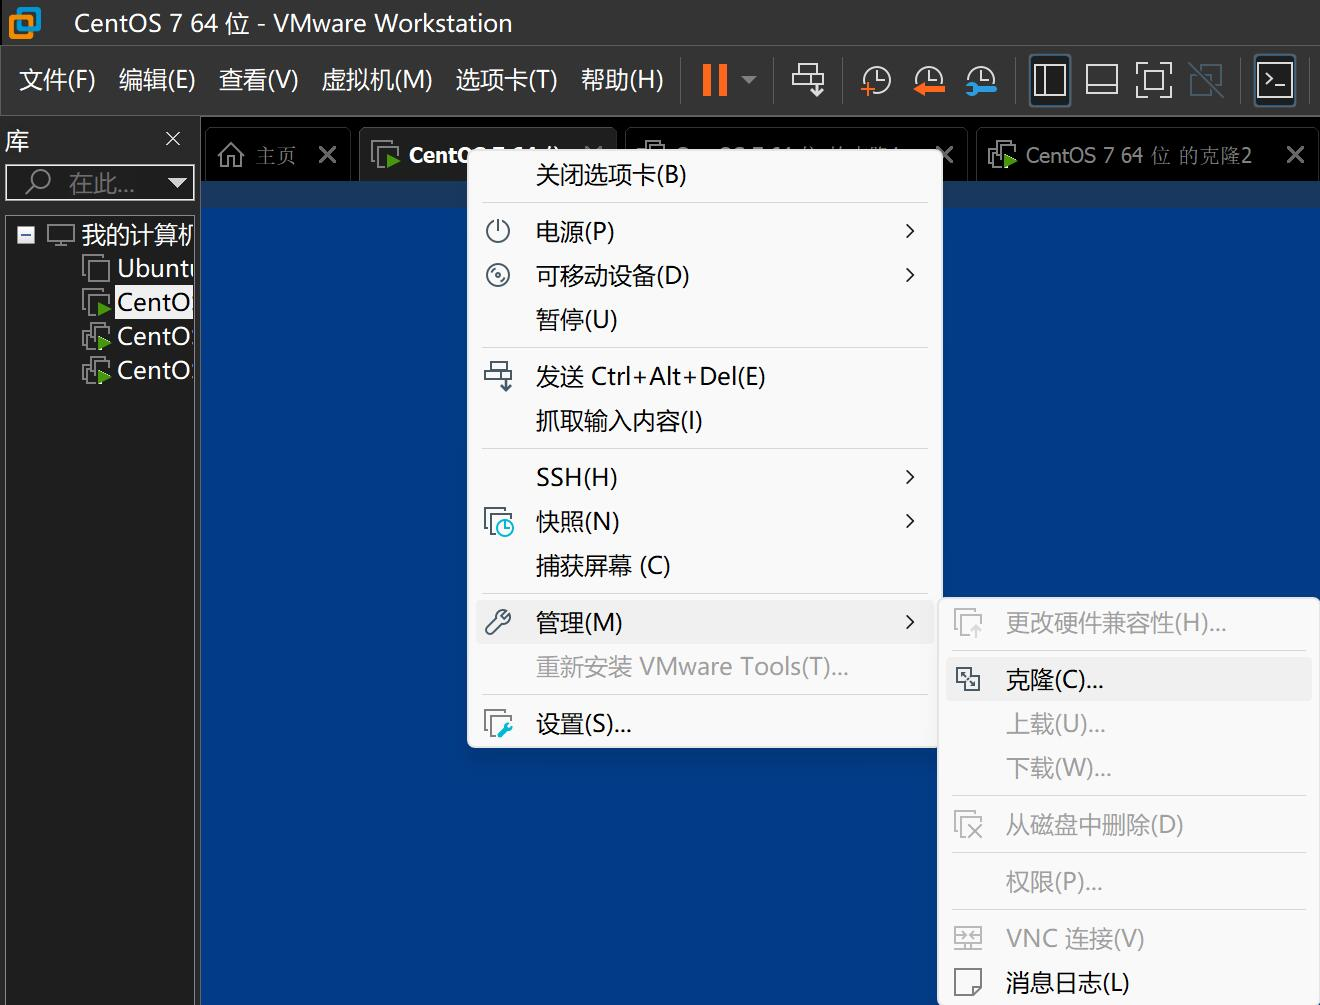
\includegraphics[width=0.9\linewidth]{figures/Clone.jpg}
  \caption{VMware 克隆虚拟机操作界面}
  \label{fig:clone_vm}
\end{figure}

\paragraph{2. 查看与配置 IP 地址}
进入虚拟机后,使用以下命令查看分配的 IP 地址:
\begin{lstlisting}[style=shell]
# 查看网卡信息
ifconfig

# 或者使用 ip 命令
ip addr
\end{lstlisting}

如需设置静态 IP,需修改网卡配置文件(以 \texttt{ifcfg-ens33} 为例):
\begin{lstlisting}[style=shell]
TYPE=Ethernet
BOOTPROTO=static
NAME=ens33
DEVICE=ens33
ONBOOT=yes

IPADDR=192.168.44.139
NETMASK=255.255.255.0
GATEWAY=192.168.44.2
DNS1=223.5.5.5
DNS2=8.8.8.8
\end{lstlisting}

修改完成后,执行以下命令重启网络服务使配置生效:
\begin{lstlisting}[style=shell]
systemctl restart network
\end{lstlisting}

\paragraph{3. 设置主机名与 hosts 文件}
为保证节点间互通,在每台虚拟机上设置唯一主机名:
\begin{lstlisting}[style=shell]
# 在 node1 上执行
hostnamectl set-hostname node1

# 在 node2 上执行  
hostnamectl set-hostname node2

# 在 node3 上执行
hostnamectl set-hostname node3
\end{lstlisting}

在所有节点的 \texttt{/etc/hosts} 文件中添加如下映射:
\begin{lstlisting}[style=shell]
192.168.44.139 node1
192.168.44.140 node2
192.168.44.141 node3
\end{lstlisting}

在 Windows 宿主机的 \texttt{C:\textbackslash Windows\textbackslash System32\textbackslash drivers\textbackslash etc\textbackslash hosts} 文件中,也需写入相同映射,确保通过主机名可以直接访问虚拟机。

\paragraph{4. 配置 SSH 免密登录}
为方便分布式管理,需要配置 SSH 免密。首先在 node1 上生成密钥对:
\begin{lstlisting}[style=shell]
ssh-keygen -t rsa
\end{lstlisting}

将生成的公钥分发至各节点:
\begin{lstlisting}[style=shell]
ssh-copy-id node1
ssh-copy-id node2
ssh-copy-id node3
\end{lstlisting}

配置完成后,可以直接通过 \texttt{ssh node2} 或 \texttt{ssh node3} 登录,而无需输入密码。

\paragraph{5. 验证网络互通}
最后,通过 \texttt{ping} 和 \texttt{ssh} 验证各节点的连通性:
\begin{lstlisting}[style=shell]
# 测试 node1 与 node2 的连通性
ping node2

# 从 node1 免密登录到 node3
ssh node3
\end{lstlisting}

若所有节点均能互通,则虚拟机与网络配置完成,可以进入 Hadoop 集群安装步骤。

\subsection{Hadoop集群配置}

以下展示对核心配置文件的修改,并解释每个配置项的意义。

\begin{lstlisting}[style=xml, caption={core-site.xml核心配置}]
<?xml version="1.0" encoding="UTF-8"?>
<?xml-stylesheet type="text/xsl" href="configuration.xsl"?>
<configuration>
    <!-- 指定HDFS的NameNode地址 -->
    <property>
        <name>fs.defaultFS</name>
        <value>hdfs://node1:9000</value>
        <description>NameNode的地址</description>
    </property>
    
    <!-- 指定Hadoop临时目录 -->
    <property>
        <name>hadoop.tmp.dir</name>
        <value>/opt/hadoop/tmp</value>
        <description>Hadoop临时文件存储目录</description>
    </property>
    
    <!-- 缓冲区大小配置 -->
    <property>
        <name>io.file.buffer.size</name>
        <value>131072</value>
        <description>文件缓冲区大小</description>
    </property>
</configuration>
\end{lstlisting}

\begin{lstlisting}[style=xml, caption={hdfs-site.xml存储配置}]
<?xml version="1.0" encoding="UTF-8"?>
<?xml-stylesheet type="text/xsl" href="configuration.xsl"?>
<configuration>
    <!-- 数据副本数量 -->
    <property>
        <name>dfs.replication</name>
        <value>3</value>
        <description>HDFS数据块副本数量</description>
    </property>
    
    <!-- NameNode数据存储路径 -->
    <property>
        <name>dfs.namenode.name.dir</name>
        <value>/opt/hadoop/data/namenode</value>
        <description>NameNode元数据存储目录</description>
    </property>
    
    <!-- DataNode数据存储路径 -->
    <property>
        <name>dfs.datanode.data.dir</name>
        <value>/opt/hadoop/data/datanode</value>
        <description>DataNode数据存储目录</description>
    </property>
    
    <!-- 数据块大小设置 -->
    <property>
        <name>dfs.blocksize</name>
        <value>134217728</value>
        <description>HDFS数据块大小(128MB)</description>
    </property>
</configuration>
\end{lstlisting}

\begin{lstlisting}[style=xml, caption={yarn-site.xml资源管理配置}]
<?xml version="1.0" encoding="UTF-8"?>
<configuration>
    <!-- ResourceManager 地址 -->
    <property>
        <name>yarn.resourcemanager.hostname</name>
        <value>node1</value>
        <description>ResourceManager主机名</description>
    </property>
    
    <!-- NodeManager 辅助服务 -->
    <property>
        <name>yarn.nodemanager.aux-services</name>
        <value>mapreduce_shuffle</value>
        <description>NodeManager辅助服务</description>
    </property>
    
    <!-- 内存分配设置 -->
    <property>
        <name>yarn.nodemanager.resource.memory-mb</name>
        <value>2048</value>
        <description>NodeManager可用内存</description>
    </property>
</configuration>
\end{lstlisting}

\begin{lstlisting}[style=xml, caption={mapred-site.xml作业配置}]
<?xml version="1.0" encoding="UTF-8"?>
<configuration>
    <!-- 指定MapReduce框架为yarn -->
    <property>
        <name>mapreduce.framework.name</name>
        <value>yarn</value>
        <description>MapReduce运行框架</description>
    </property>
    
    <!-- JobHistory Server地址 -->
    <property>
        <name>mapreduce.jobhistory.address</name>
        <value>node1:10020</value>
        <description>历史服务器地址</description>
    </property>
    
    <!-- JobHistory Web地址 -->
    <property>
        <name>mapreduce.jobhistory.webapp.address</name>
        <value>node1:19888</value>
        <description>历史服务器Web界面</description>
    </property>
</configuration>
\end{lstlisting}

最后,在 \texttt{\$HADOOP\_HOME/etc/hadoop/workers} 文件中指定工作节点:
\begin{lstlisting}[style=shell, caption={workers配置}]
node1
node2  
node3
\end{lstlisting}

\subsection{HBase集群配置}

在完成 Hadoop 集群部署之后,需要进一步安装并配置 HBase,使其能够依赖 HDFS 进行存储,并借助 ZooKeeper 进行分布式协调。

\paragraph{1. 解压与环境变量配置}
在所有节点下载并解压 HBase 安装包,然后在 \texttt{/etc/profile} 中配置 HBase 环境变量:
\begin{lstlisting}[style=shell]
export HBASE_HOME=/opt/hbase-2.1.0
export PATH=$PATH:$HBASE_HOME/bin
\end{lstlisting}

保存后执行 \texttt{source /etc/profile} 使配置立即生效。

\paragraph{2. 修改 hbase-site.xml}
进入 \texttt{\$HBASE\_HOME/conf} 目录,编辑 \texttt{hbase-site.xml} 文件,主要配置如下:
\begin{lstlisting}[style=xml, caption={hbase-site.xml配置示例}]
<?xml version="1.0" encoding="UTF-8"?>
<configuration>
    <!-- HBase 在 HDFS 上的存储目录 -->
    <property>
        <name>hbase.rootdir</name>
        <value>hdfs://node1:9000/hbase</value>
    </property>

    <!-- HBase 以分布式模式运行 -->
    <property>
        <name>hbase.cluster.distributed</name>
        <value>true</value>
    </property>

    <!-- ZooKeeper 集群地址 -->
    <property>
        <name>hbase.zookeeper.quorum</name>
        <value>node1,node2,node3</value>
    </property>

    <!-- Write-Ahead Log (WAL) 存储方式 -->
    <property>
        <name>hbase.wal.provider</name>
        <value>filesystem</value>
    </property>

    <!-- HBase 临时目录 -->
    <property>
        <name>hbase.tmp.dir</name>
        <value>/opt/hbase/tmp</value>
    </property>
</configuration>
\end{lstlisting}

\paragraph{3. 修改 regionservers 文件}
在 \texttt{\$HBASE\_HOME/conf/regionservers} 文件中,列出所有参与 HBase 的工作节点:
\begin{lstlisting}[style=shell, caption={regionservers 配置}]
node1
node2
node3
\end{lstlisting}

\paragraph{4. hbase-env.sh 配置}
在 \texttt{hbase-env.sh} 文件中,指定 HBase 的 Java 环境:
\begin{lstlisting}[style=shell]
export JAVA_HOME=/usr/java/jdk1.8.0_241
\end{lstlisting}

\paragraph{5. ZooKeeper 与 HBase 关系说明}
HBase 内部依赖 ZooKeeper 进行协调,但若集群已单独部署 ZooKeeper,可以通过上述配置直接指定外部 ZooKeeper 集群地址。否则,HBase 会默认使用自带的 ZooKeeper。

\paragraph{6. 验证配置}
完成上述配置后,在 node1 上执行:
\begin{lstlisting}[style=shell]
start-hbase.sh
\end{lstlisting}

然后在 node1 上运行:
\begin{lstlisting}[style=shell]
hbase shell
\end{lstlisting}

若能进入 HBase Shell,说明配置成功。之后可以通过 \texttt{list}、\texttt{create}、\texttt{scan} 等命令进一步验证 HBase 的功能。


\subsection{集群启动与验证}

在完成 Hadoop、ZooKeeper 与 HBase 的配置后,需要按顺序启动各个服务,并验证其是否正常运行。

\paragraph{1. 启动 HDFS 与 YARN}
首先在 node1 节点执行以下命令启动 HDFS 与 YARN 服务:
\begin{lstlisting}[style=shell]
# 启动 HDFS
start-dfs.sh

# 启动 YARN
start-yarn.sh
\end{lstlisting}

执行完成后,可通过以下命令检查进程是否正常:
\begin{lstlisting}[style=shell]
jps
\end{lstlisting}

在正常情况下,NameNode、SecondaryNameNode、DataNode、ResourceManager、NodeManager 等进程应全部启动。

\begin{figure}[H]
  \centering
  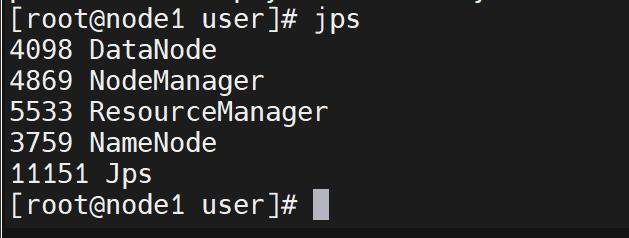
\includegraphics[width=0.8\linewidth]{figures/jps_node1.png}
  \caption{node1 节点 jps 进程验证结果(包含 NameNode、ResourceManager 等)}
  \label{fig:jps_node1}
\end{figure}

\begin{figure}[H]
  \centering
  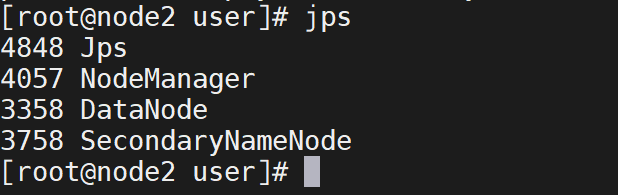
\includegraphics[width=0.8\linewidth]{figures/jps_node2.png}
  \caption{node2 节点 jps 进程验证结果(包含 SecondaryNameNode、NodeManager 等)}
  \label{fig:jps_node2}
\end{figure}

\begin{figure}[H]
  \centering
  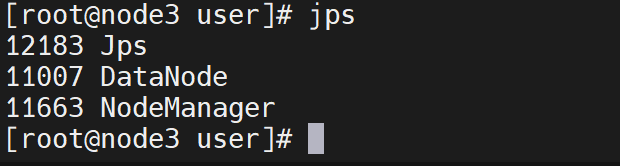
\includegraphics[width=0.8\linewidth]{figures/jps_node3.png}
  \caption{node3 节点 jps 进程验证结果(包含 DataNode、NodeManager 等)}
  \label{fig:jps_node3}
\end{figure}


\paragraph{2. 启动 ZooKeeper 集群}
在 node1、node2、node3 节点分别执行以下命令,启动 ZooKeeper 服务:
\begin{lstlisting}[style=shell]
zkServer.sh start
\end{lstlisting}

使用以下命令查看 ZooKeeper 状态:
\begin{lstlisting}[style=shell]
zkServer.sh status
\end{lstlisting}

其中 node1 显示为 \texttt{leader},node2 与 node3 显示为 \texttt{follower} 即为正常。

\paragraph{3. 启动 HBase}
在 node1 上执行以下命令启动 HBase 服务:
\begin{lstlisting}[style=shell]
start-hbase.sh
\end{lstlisting}

随后可通过以下命令验证进程:
\begin{lstlisting}[style=shell]
jps
\end{lstlisting}

若看到 HMaster 与 HRegionServer 等进程,说明 HBase 启动成功。

\begin{figure}[H]
  \centering
  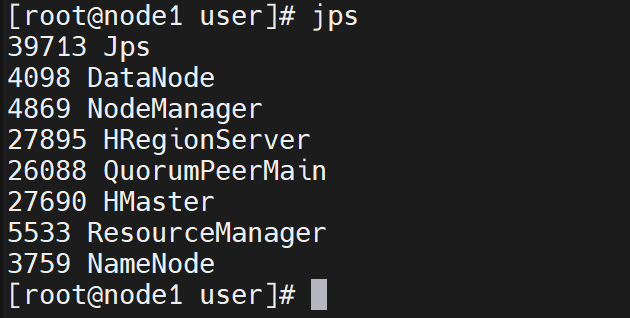
\includegraphics[width=0.8\linewidth]{figures/jps_hbase_node1.png}
  \caption{node1 节点 jps 进程验证结果(包含 HMaster、HRegionServer 等)}
  \label{fig:jps_hbase_node1}
\end{figure}

\begin{figure}[H]
  \centering
  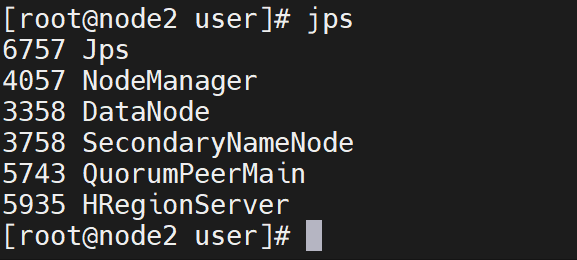
\includegraphics[width=0.8\linewidth]{figures/jps_hbase_node2.png}
  \caption{node2 节点 jps 进程验证结果(包含 SecondaryNameNode、HRegionServer 等)}
  \label{fig:jps_hbase_node2}
\end{figure}

\begin{figure}[H]
  \centering
  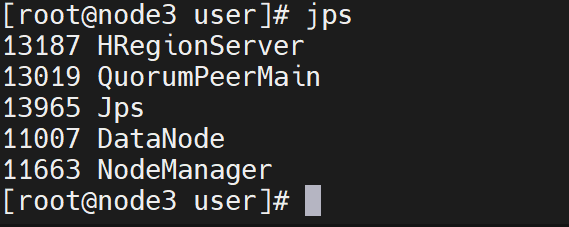
\includegraphics[width=0.8\linewidth]{figures/jps_hbase_node3.png}
  \caption{node3 节点 jps 进程验证结果(包含 HRegionServer 等)}
  \label{fig:jps_hbase_node3}
\end{figure}

\paragraph{4. Web UI 验证}
各组件启动成功后,可以通过 Web 界面进行验证:
\begin{itemize}
  \item HDFS NameNode 管理界面:\url{http://node1:9870}
  \item YARN ResourceManager 界面:\url{http://node1:8088}
  \item HBase Master 界面:\url{http://node1:16010}
\end{itemize}

通过浏览器访问上述地址,可以查看各个服务的运行状态及任务执行情况。

\begin{figure}[H]
  \centering
  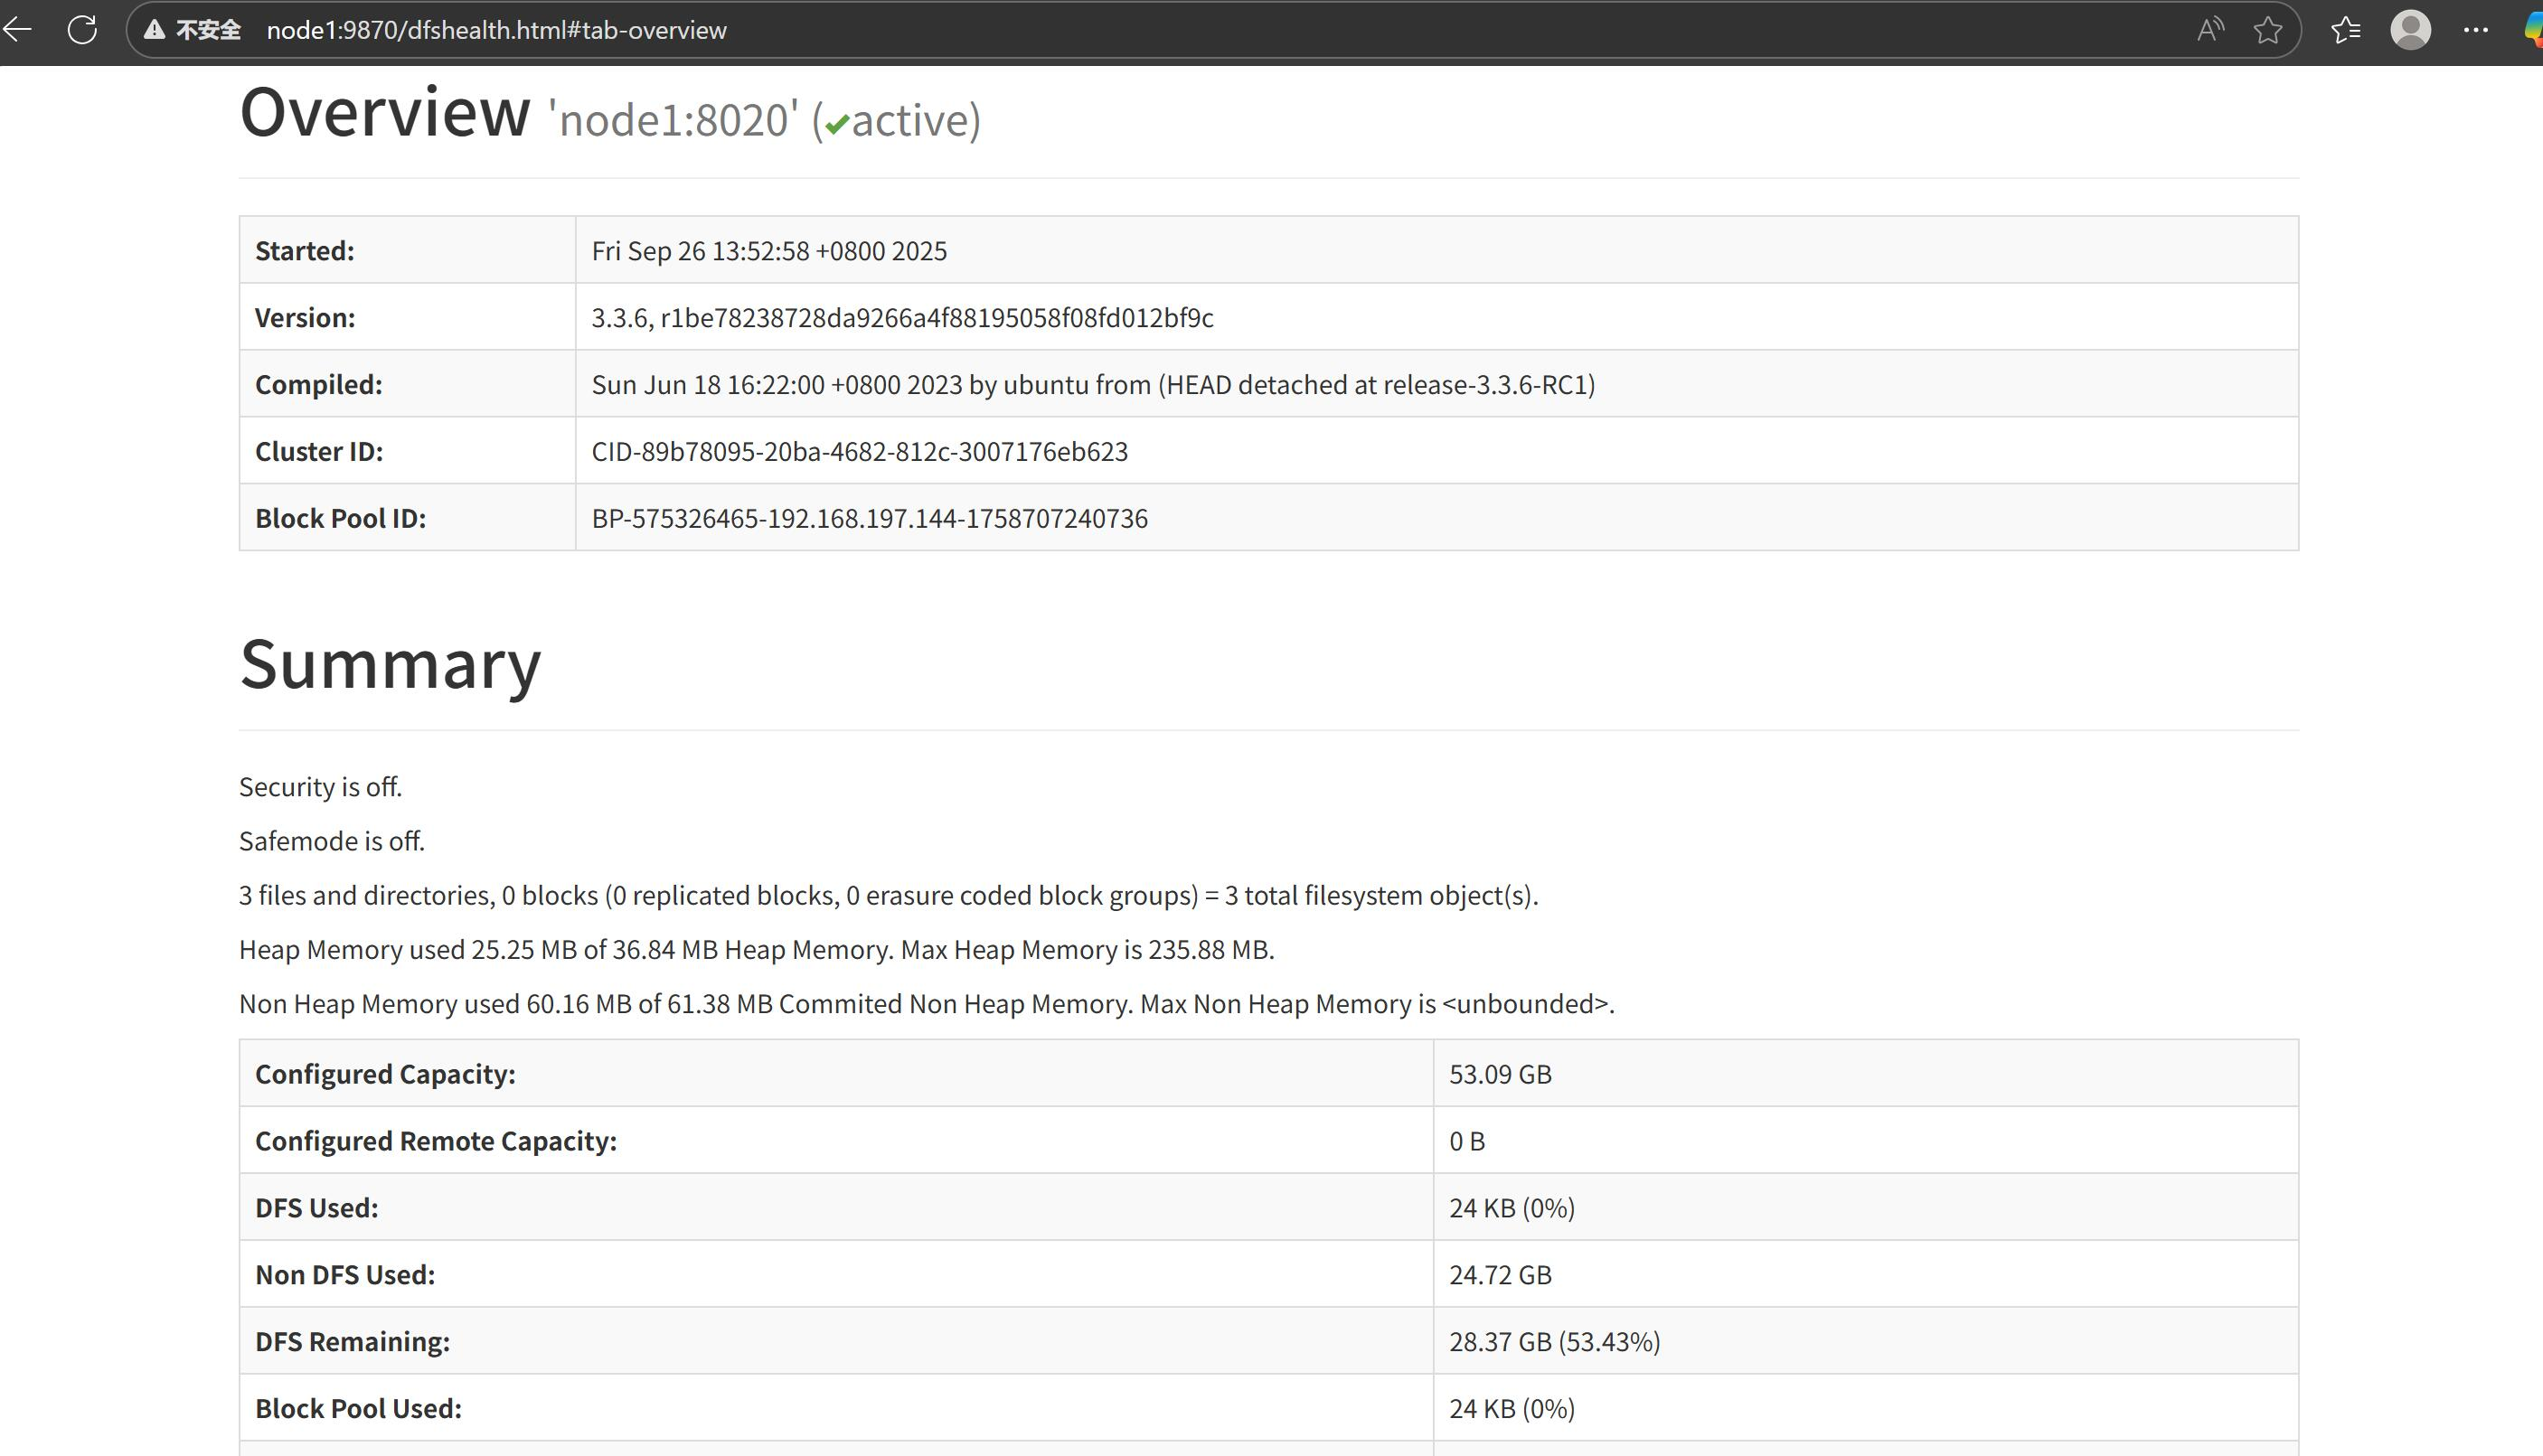
\includegraphics[width=0.9\linewidth]{figures/web_hdfs.jpg}
  \caption{HDFS NameNode Web 界面 (http://node1:9870)}
  \label{fig:web_hdfs}
\end{figure}

\begin{figure}[H]
  \centering
  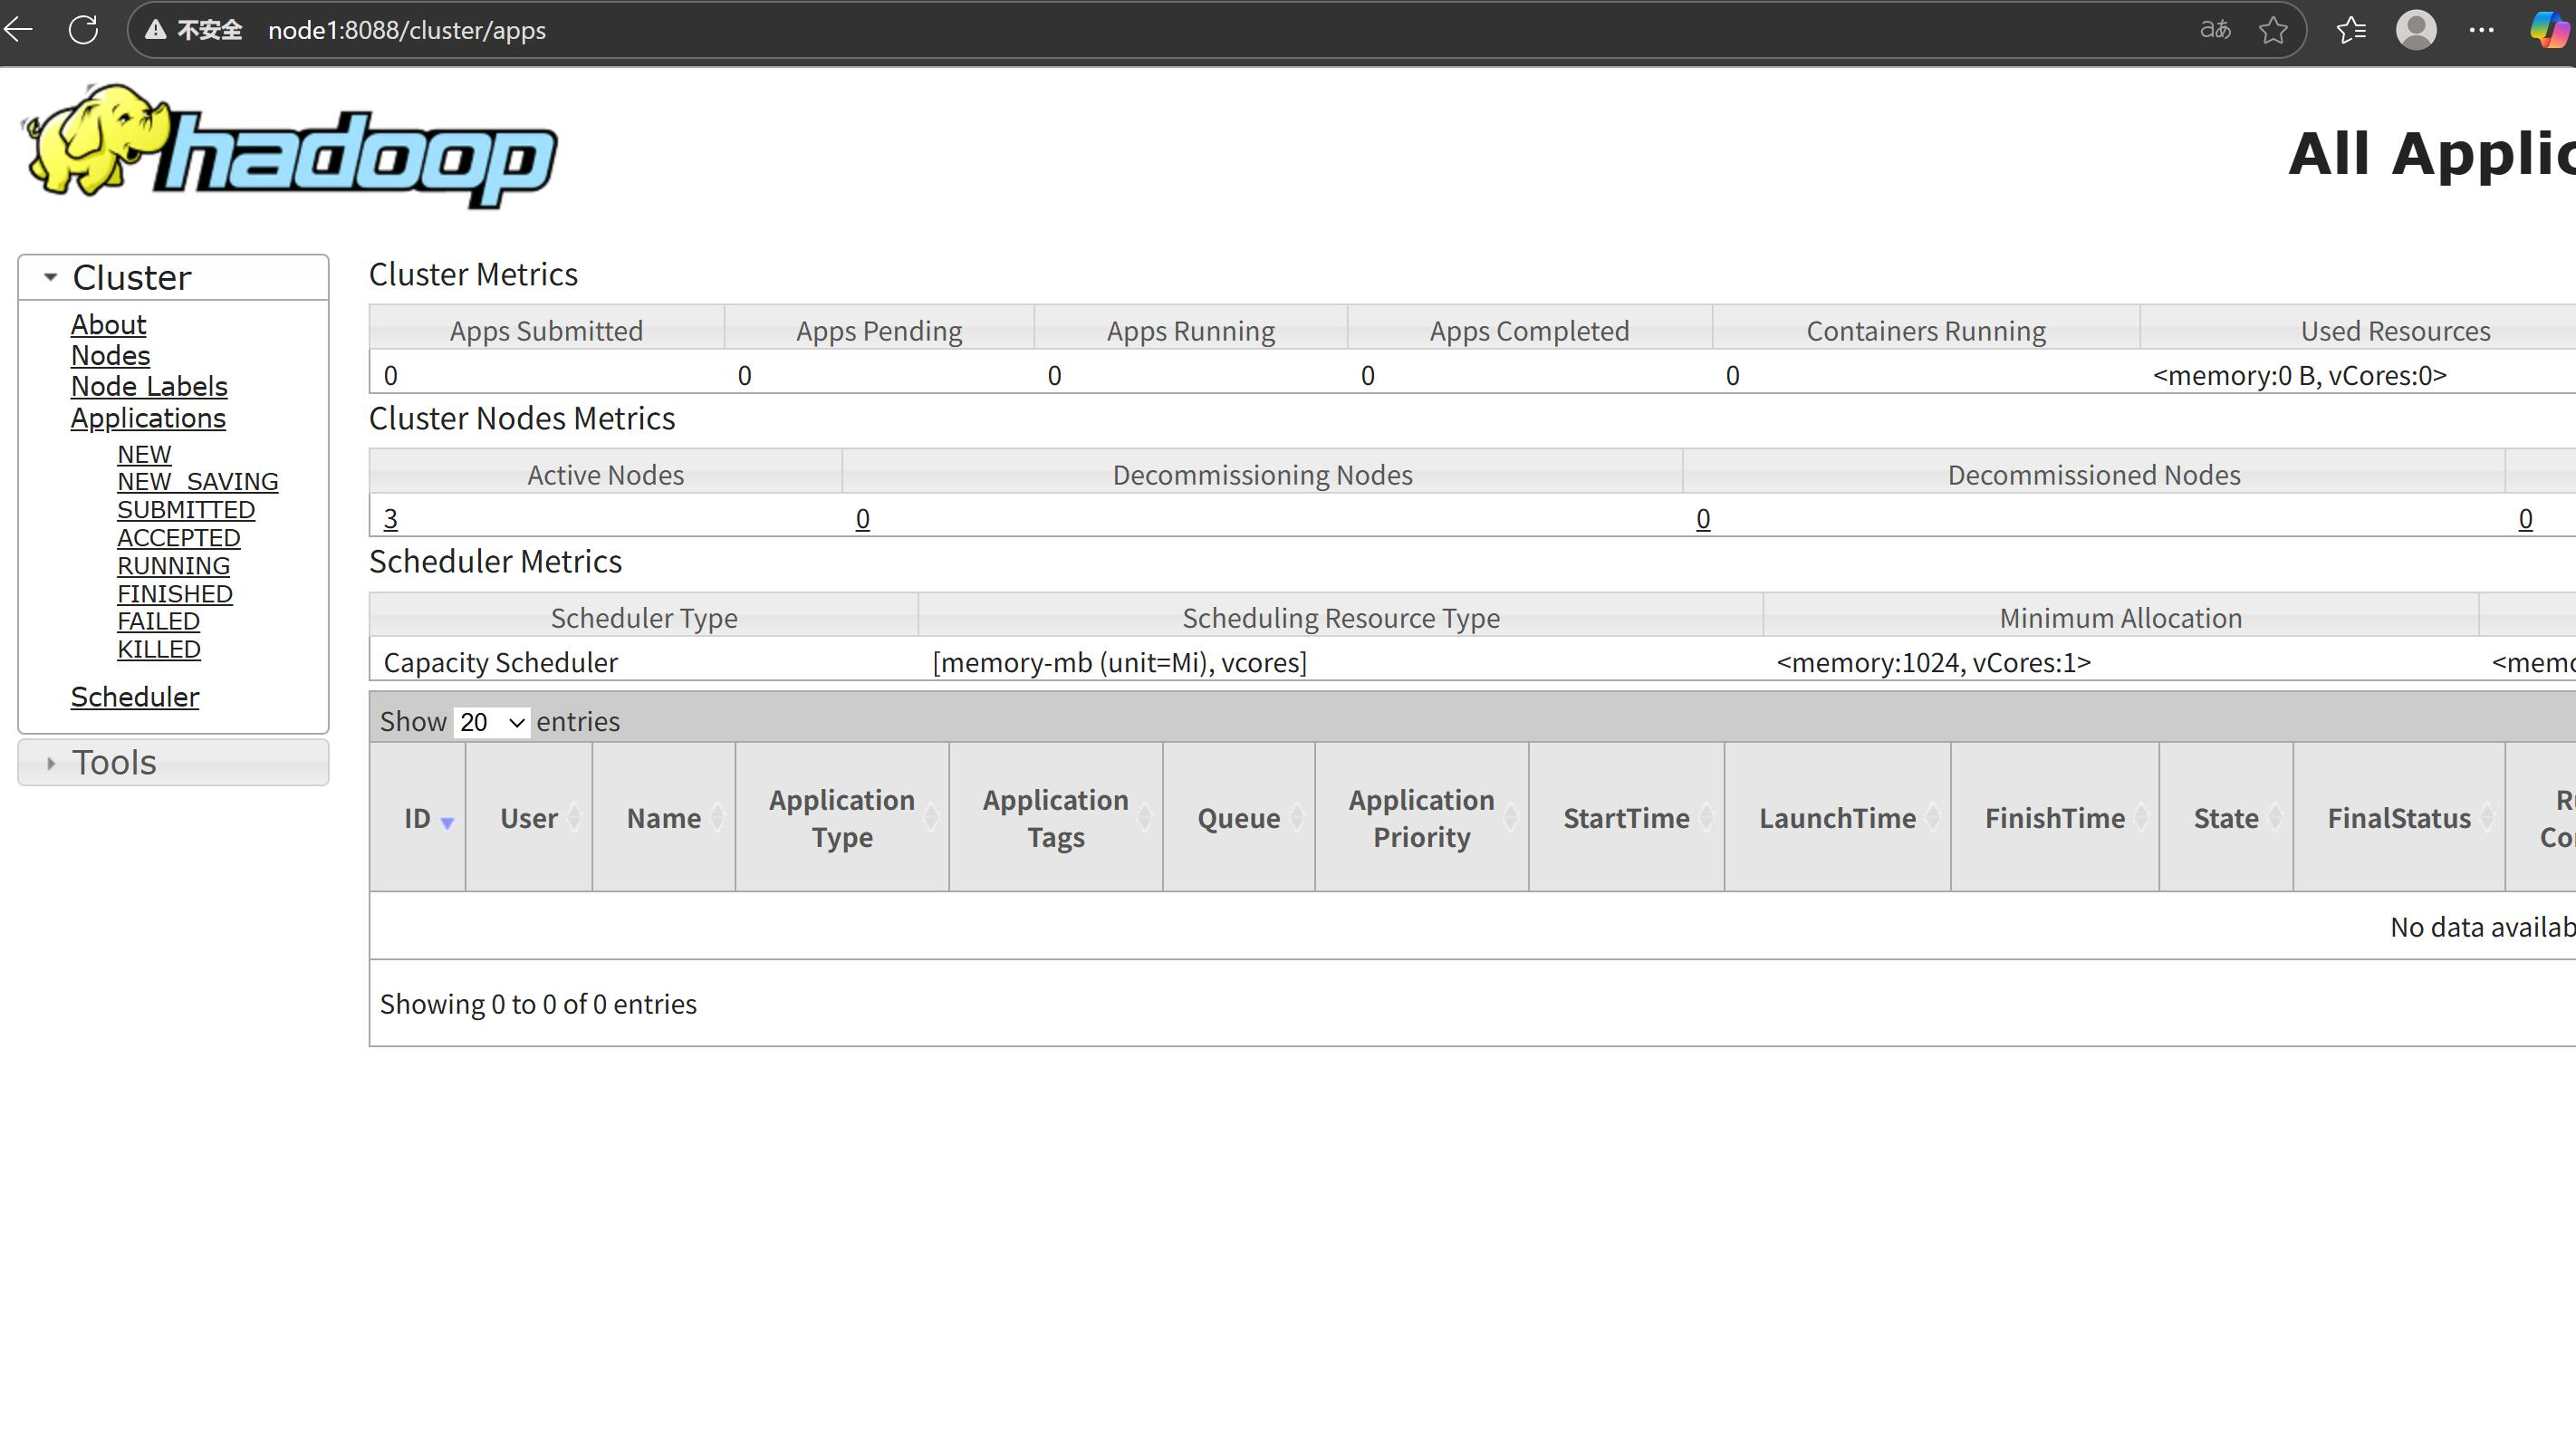
\includegraphics[width=0.9\linewidth]{figures/web_yarn.jpg}
  \caption{YARN ResourceManager Web 界面 (http://node1:8088)}
  \label{fig:web_yarn}
\end{figure}

\begin{figure}[H]
  \centering
  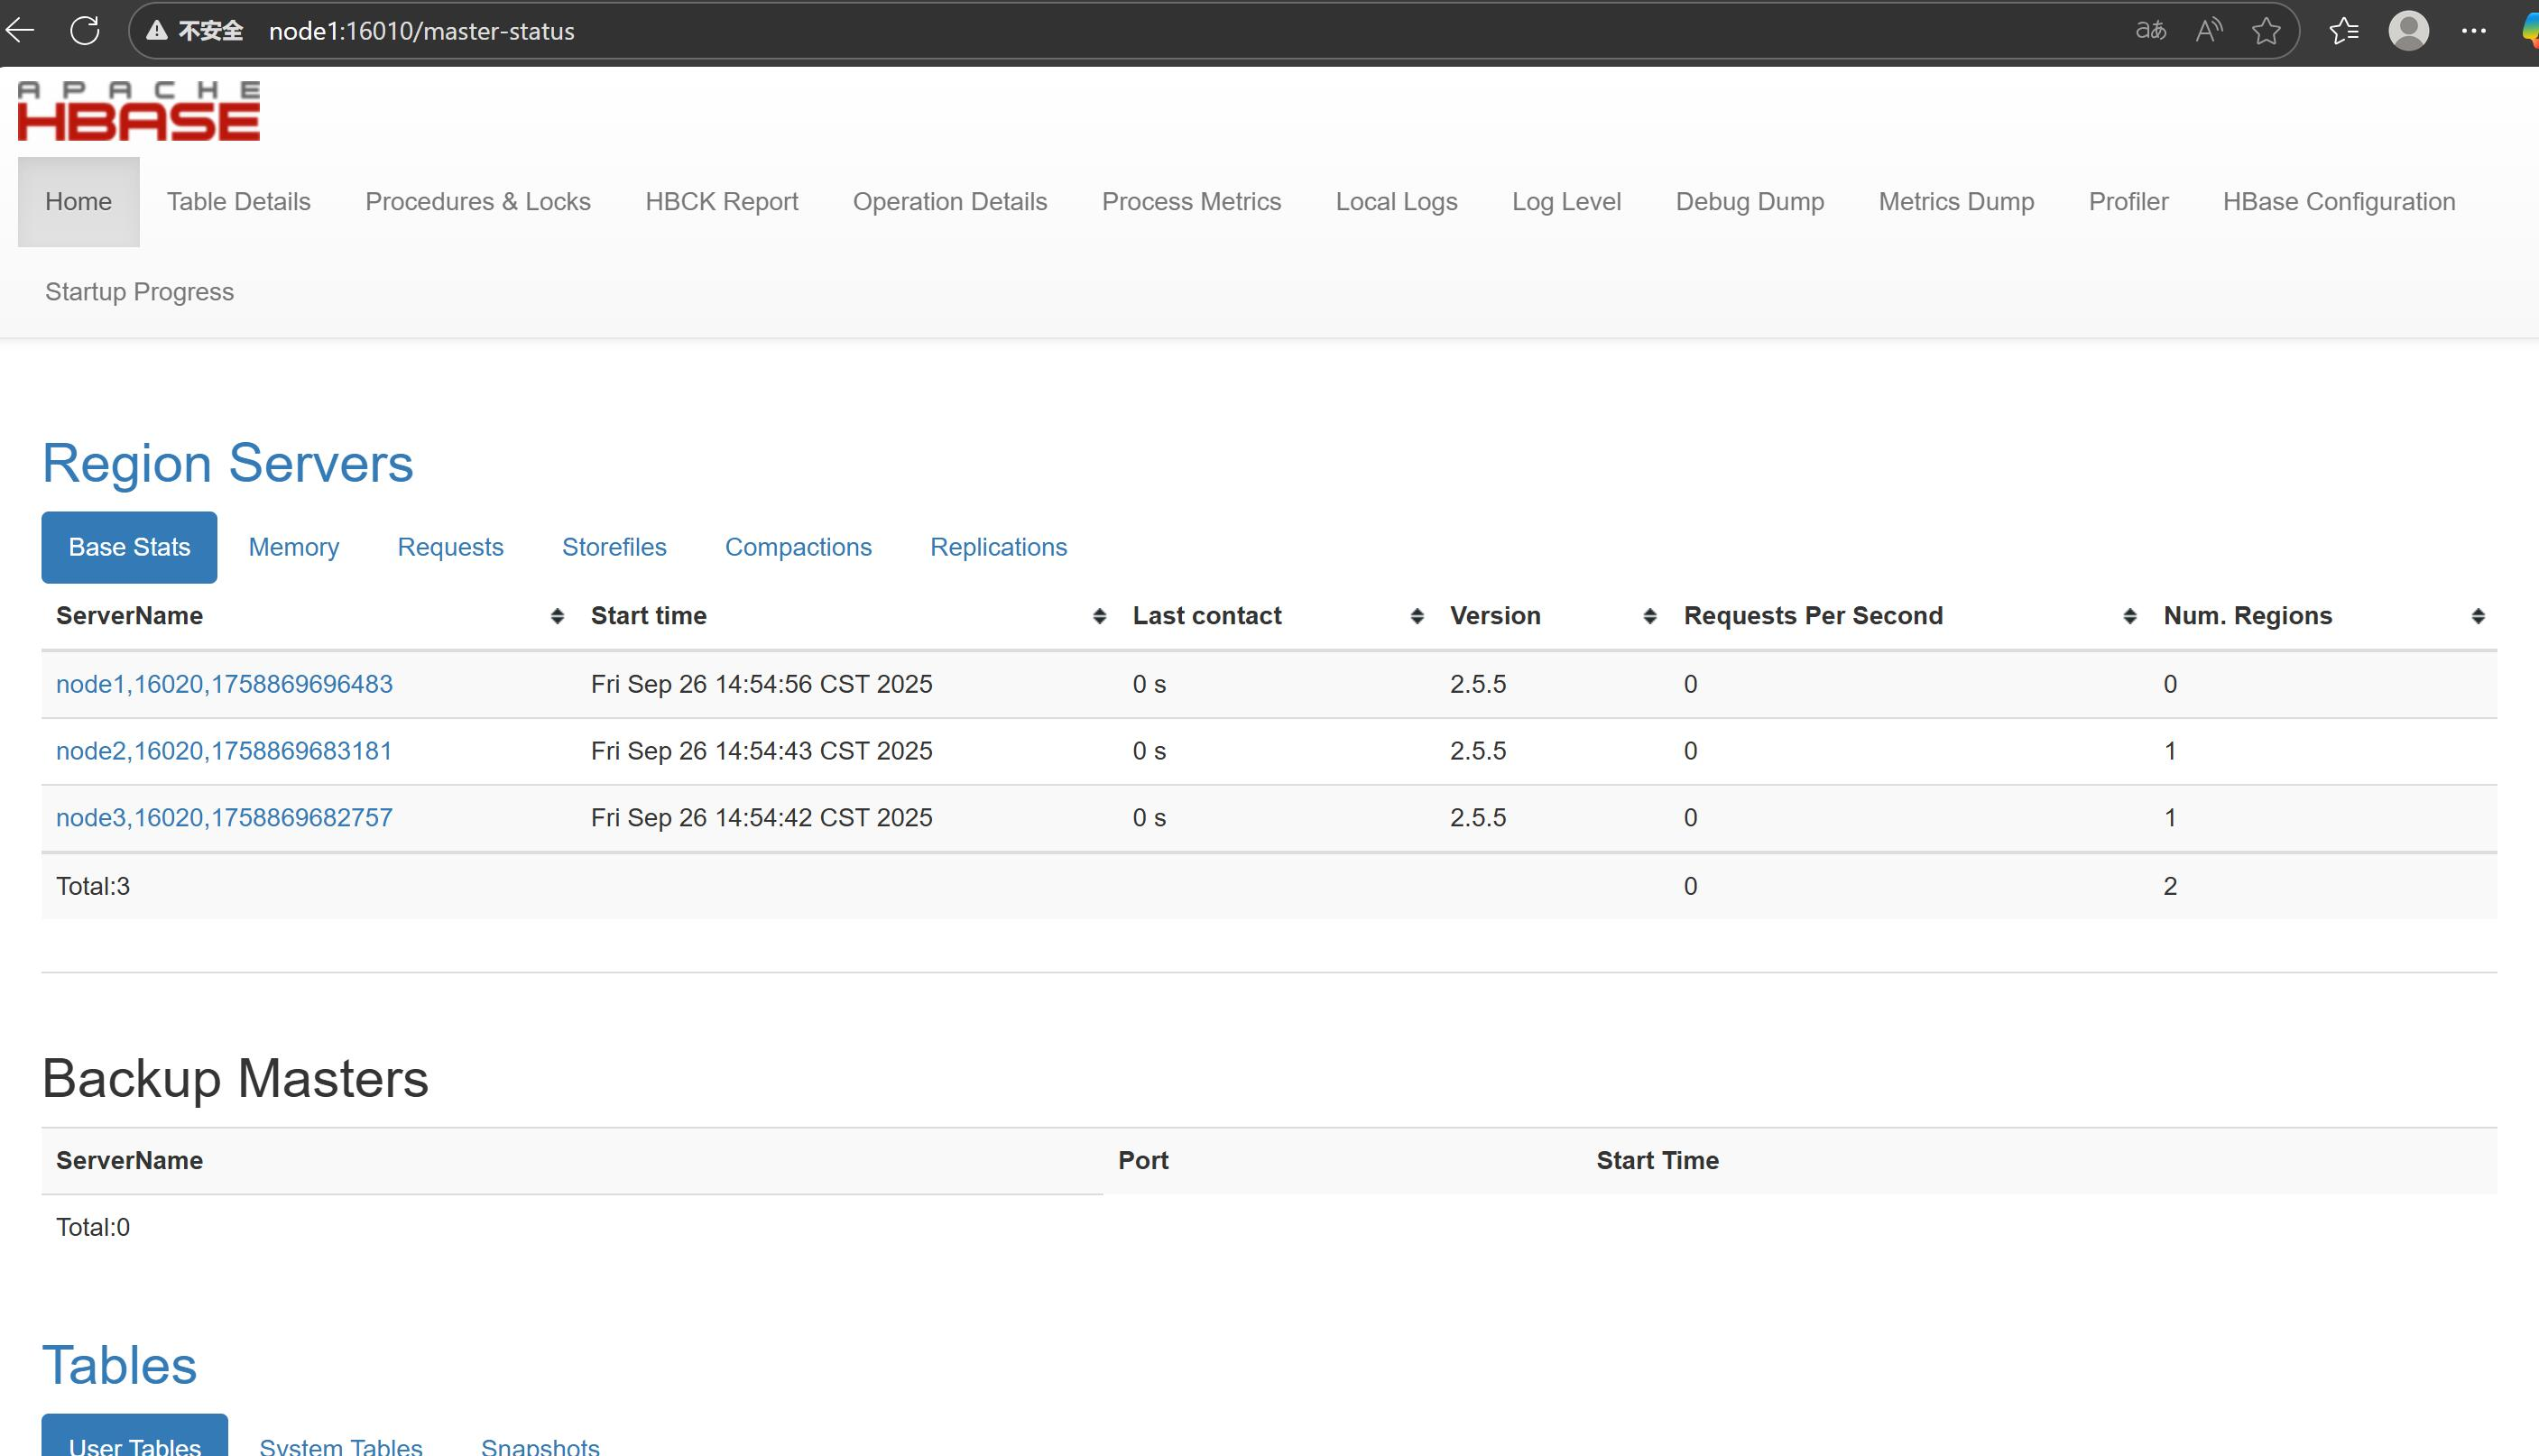
\includegraphics[width=0.9\linewidth]{figures/web_hbase.jpg}
  \caption{HBase Master Web 界面 (http://node1:16010)}
  \label{fig:web_hbase}
\end{figure}

\paragraph{5. HBase Shell 验证}
最后进入 HBase Shell,执行以下命令验证功能:
\begin{lstlisting}[style=shell]
hbase shell

# 在 HBase Shell 中输入
list
\end{lstlisting}

若能够正确输出当前已有的表,说明 HBase 与 Hadoop 集群已成功运行。

\section{实验过程与实现}

\subsection{数据准备}
本次实验所使用的原始数据集为 \texttt{sentences.txt},大小约为 1.43GB,数据量较大。如果直接将该文件作为 MapReduce 的输入,单节点读取和处理的效率较低。因此,在实验开始前,我们首先对原始文件进行分割处理,使其能够更好地并行分布到各个节点进行计算。

为了实现数据分割,我们编写了一个 Python 脚本,按照每 10000 行划分为一个子文件。其核心代码如下所示:

\begin{lstlisting}[language=Python, caption={文件分割脚本}]
def split_file(input_filename, lines_per_file=10000):
    # 打开输入文件
    with open(input_filename, 'r', encoding='utf-8') as input_file:
        file_count = 1      # 输出文件计数器
        current_output = None
        
        for line_number, line in enumerate(input_file, 1):
            # 每当开始新文件时,关闭旧文件并创建新文件
            if line_number % lines_per_file == 1:
                if current_output:
                    current_output.close()
                output_filename = f"split_{file_count}.txt"
                current_output = open(output_filename, 'w', encoding='utf-8')
                file_count += 1
            # 将当前行写入输出文件
            current_output.write(line)
        
        if current_output:
            current_output.close()

# 使用函数对 sentences.txt 进行分割
split_file('./sentences.txt')
\end{lstlisting}

运行该脚本后,原始文件被拆分为多个大小约为 1.4MB 的子文件,如图~\ref{fig:splitfiles} 所示。每个子文件包含约 10000 行数据,最终共生成 940 个分片文件,分别命名为 \texttt{split\_1.txt} 至 \texttt{split\_940.txt}。

\begin{figure}[H]
  \centering
  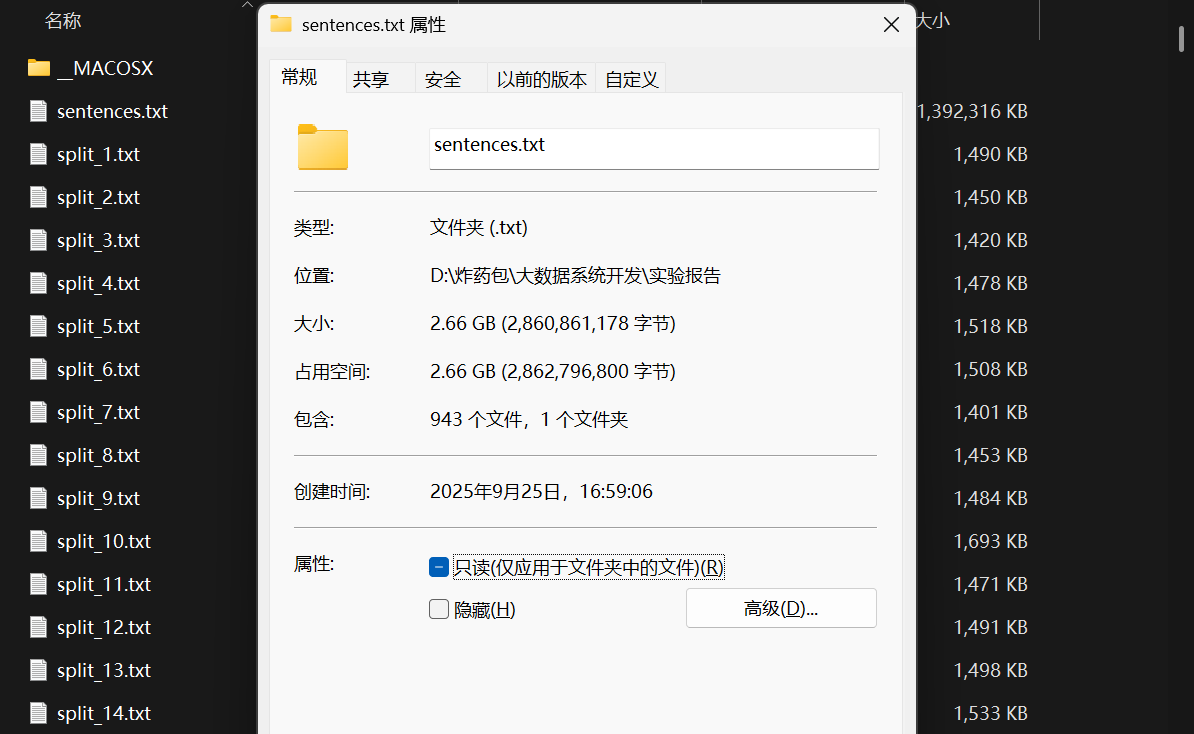
\includegraphics[width=0.9\linewidth]{figures/Step1_FileSplit.png}
  \caption{数据集拆分结果}
  \label{fig:splitfiles}
\end{figure}

接下来,需要将这些拆分后的文件上传到 HDFS,以便后续的 MapReduce 程序进行处理。首先,在 HDFS 中创建一个用于存放实验输入数据的目录:

\begin{lstlisting}[style=shell]
hdfs dfs -mkdir -p /user/input
\end{lstlisting}

然后,将拆分好的文件批量上传至该目录:

\begin{lstlisting}[style=shell]
hdfs dfs -put split_*.txt /user/input
\end{lstlisting}

至此,实验所需的数据已经准备完毕,HDFS 中的目录结构如图~\ref{fig:hdfs_input} 所示。

\begin{figure}[H]
  \centering
  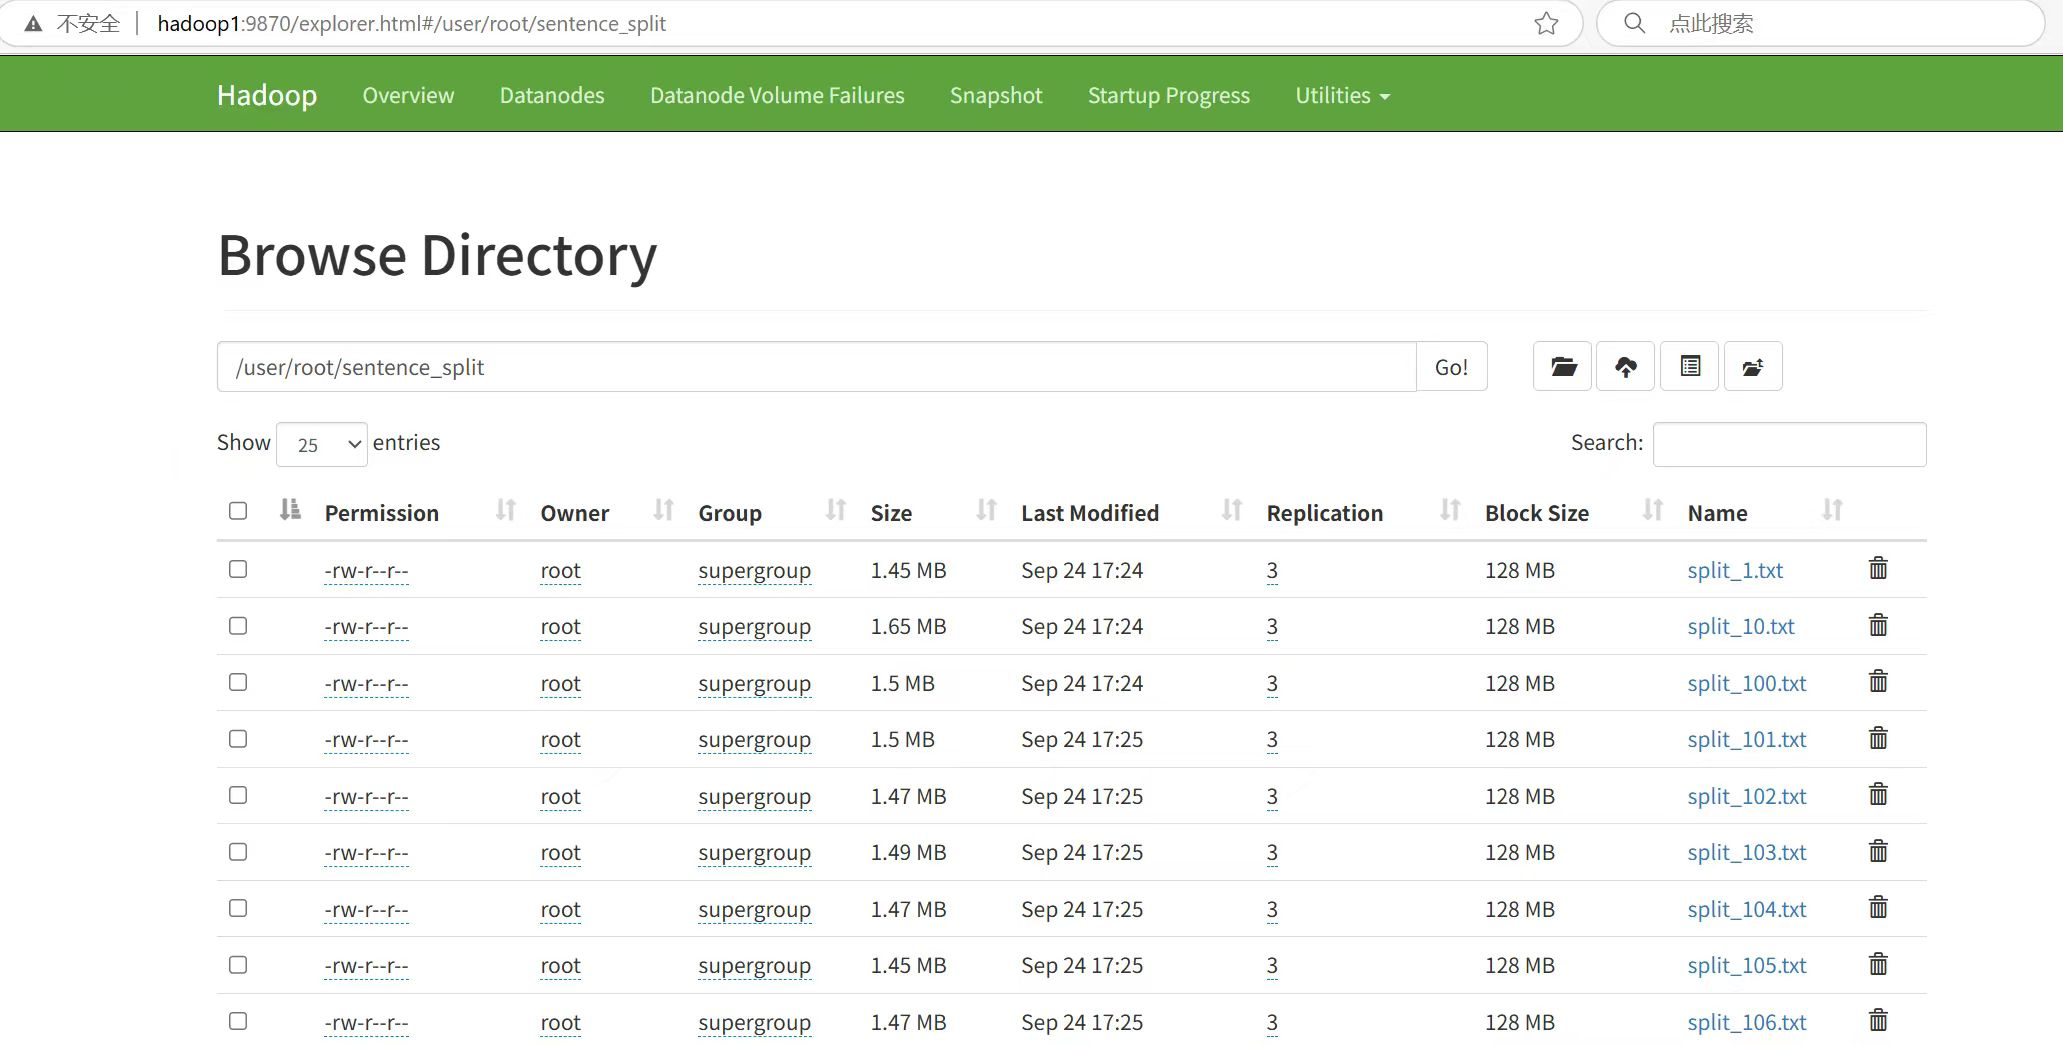
\includegraphics[width=0.9\linewidth]{figures/Step2_HDFSInput.png}
  \caption{上传至 HDFS 的数据目录}
  \label{fig:hdfs_input}
\end{figure}

\subsection{核心算法与代码实现}

\subsubsection{Mapper实现}

Mapper 的核心任务是对输入的文本数据进行分词,并记录单词出现的位置信息。在本实验中,位置信息不仅包括单词本身,还包含该单词所在的文件名,从而为后续构建倒排索引做好准备。

\begin{lstlisting}[style=java, caption={Mapper核心代码}]
public static class Map extends Mapper<Object, Text, Text, Text> {
    private Text keyInfo = new Text();
    private Text valueInfo = new Text();
    private FileSplit split;

    public void map(Object key, Text value, Context context) 
            throws IOException, InterruptedException {
        split = (FileSplit) context.getInputSplit();
        StringTokenizer itr = new StringTokenizer(value.toString());
        while (itr.hasMoreTokens()) {
            // 获取当前处理的文件名
            String fileName = split.getPath().getName();
            // 将单词与文件名拼接作为key
            keyInfo.set(itr.nextToken() + ":" + fileName);
            // 值固定为1,表示出现一次
            valueInfo.set("1");
            // 输出<单词:文件名, 1>
            context.write(keyInfo, valueInfo);
        }
    }
}
\end{lstlisting}

在上述实现中,\texttt{map()} 函数的处理逻辑如下:
\begin{itemize}
  \item 通过 \texttt{FileSplit} 获取当前正在处理的文件名,用于标识单词的来源文件。
  \item 使用 \texttt{StringTokenizer} 对输入行进行分词,逐个提取单词。
  \item 将单词与文件名拼接形成新的键(\texttt{word:filename}),对应的值统一设置为 \texttt{1},表示该单词在该文件中出现了一次。
  \item 通过 \texttt{context.write()} 输出键值对,交由框架传递给后续的 \texttt{Combine} 或 \texttt{Reduce} 阶段。
\end{itemize}

这样处理的好处在于:在 Map 阶段就已经将单词与所在文件建立了联系,为后续统计和去重操作奠定了基础。最终目标是能够在 HBase 中形成倒排索引表,使得任意一个单词可以快速定位到其所在的文件集合。

\subsubsection{Reducer实现}

Reducer 的主要任务是将 Map 阶段输出的 \texttt{<单词, 文件编号>} 进行汇总,最终生成倒排索引,并写入到 HBase 表中。不同于传统的 MapReduce 将结果输出到 HDFS,本实验通过 \texttt{TableReducer} 类直接将结果存储到 HBase 的指定列族和列中。

\begin{lstlisting}[style=java, caption={Reducer核心代码}]
public static class InvertedIndexReducer 
        extends TableReducer<Text, Text, ImmutableBytesWritable> {
    
    @Override
    protected void reduce(Text key, Iterable<Text> values, Context context) 
            throws IOException, InterruptedException {
        // 用于存储所有文件编号
        List<String> fileList = new ArrayList<>();
        
        for (Text v : values) {
            String fileNum = v.toString();
            // 避免重复,将相同文件编号只保存一次
            if (!fileList.contains(fileNum)) {
                fileList.add(fileNum);
            }
        }
        
        // 将结果拼接成以逗号分隔的字符串
        StringBuilder sb = new StringBuilder();
        for (String f : fileList) {
            sb.append(f).append(",");
        }
        // 去掉最后一个多余的逗号
        String result = sb.substring(0, sb.length() - 1);
        
        // 构建Put对象:RowKey 为单词
        Put put = new Put(Bytes.toBytes(key.toString()));
        // 写入列族col_family,列名info
        put.addColumn(Bytes.toBytes("col_family"), 
                      Bytes.toBytes("info"), 
                      Bytes.toBytes(result));
        
        // 输出到HBase
        context.write(null, put);
    }
}
\end{lstlisting}

在上述实现中,\texttt{reduce()} 函数的核心逻辑如下:
\begin{itemize}
  \item 接收来自 Map 阶段的所有值(文件编号),这些值表示某个单词出现过的文件。
  \item 使用 \texttt{List<String>} 对文件编号进行去重,避免重复计入同一文件。
  \item 将所有文件编号拼接成一个以逗号分隔的字符串,例如 \texttt{''1,3,5''},表示该单词出现在 1、3、5 号文件中。
  \item 构造 HBase 的 \texttt{Put} 对象,以单词作为行键(RowKey),在列族 \texttt{col\_family} 下的列 \texttt{info} 中写入拼接后的文件编号列表。
  \item 通过 \texttt{context.write()} 方法将结果直接写入 HBase 表,实现单词到文件编号集合的倒排索引存储。
\end{itemize}

与传统 MapReduce 输出到 HDFS 不同,本实验使用 \texttt{TableReducer} 将结果直接与 HBase 集成。这不仅简化了数据落地的流程,还为后续的数据查询和分析提供了高效的支持:只需在 HBase 中查询某个单词对应的行键,即可快速获得该单词出现过的所有文件编号。

\subsubsection{Driver实现}

Driver 部分是整个 MapReduce 程序的入口,用于配置作业运行环境、指定 Mapper 与 Reducer 类、设置输入输出路径等。本实验的 Driver 还负责调用 HBase 提供的工具类,使 MapReduce 的结果直接写入到 HBase 表中。

\begin{lstlisting}[style=java, caption={Driver核心代码}]
public static void main(String[] args) 
        throws IOException, ClassNotFoundException, InterruptedException {
    
    // 1. 创建 Hadoop 与 HBase 的配置对象
    Configuration conf = HBaseConfiguration.create();
    
    // 2. 解析命令行参数,获取输入路径
    String[] otherArgs = new GenericOptionsParser(conf, args)
                             .getRemainingArgs();
    
    // 3. 创建 Job 实例
    Job job = Job.getInstance(conf, "InvertedIndex");
    job.setJarByClass(InvertedIndex.class);
    
    // 4. 设置 Mapper 与 Reducer
    job.setMapperClass(MyMapper.class);
    job.setReducerClass(MyReducer.class);
    
    job.setMapOutputKeyClass(Text.class);
    job.setMapOutputValueClass(Text.class);
    
    // 5. 将输出结果写入到 HBase 表 test_table
    TableMapReduceUtil.initTableReducerJob(
        "test_table",          // HBase表名
        MyReducer.class,       // Reducer类
        job
    );
    
    // 6. 指定输入路径(HDFS 上的数据文件)
    FileInputFormat.addInputPath(job, new Path(otherArgs[0]));
    
    // 7. 提交任务并等待执行完成
    System.exit(job.waitForCompletion(true) ? 0 : 1);
}
\end{lstlisting}

在上述代码中,Driver 的关键逻辑如下:
\begin{enumerate}
  \item 使用 \texttt{HBaseConfiguration.create()} 生成配置对象,从而支持与 HBase 的集成。
  \item 通过 \texttt{GenericOptionsParser} 解析命令行参数,获取 MapReduce 输入数据所在的 HDFS 路径。
  \item 设置作业的核心类 \texttt{InvertedIndex},并指定对应的 Mapper 与 Reducer 类。
  \item 调用 \texttt{TableMapReduceUtil.initTableReducerJob()},将 Reducer 的输出直接写入到 HBase 表 \texttt{test\_table},而不是传统的 HDFS 文件。
  \item 通过 \texttt{FileInputFormat.addInputPath()} 指定输入路径,从而让 Hadoop 在 HDFS 中读取拆分后的语料文件。
  \item 最后调用 \texttt{job.waitForCompletion(true)} 提交作业并阻塞等待执行结果。
\end{enumerate}

通过这种方式,本实验实现了从 HDFS 输入 → MapReduce 计算 → HBase 存储的完整大数据处理流程。相比于将结果写回 HDFS 文件,再导入数据库的方式,这种集成方案大大简化了处理链路,体现了 Hadoop 与 HBase 的紧密结合。

\subsection{程序打包与执行}

在完成核心代码编写后,需要将项目打包为 JAR 文件,以便提交给 Hadoop 集群执行。本实验采用 \textbf{Maven} 进行项目管理与打包,执行以下命令即可生成可运行的 JAR 包:

\begin{lstlisting}[style=shell]
mvn clean package -DskipTests
\end{lstlisting}

上述命令会在 \texttt{target/} 目录下生成 \texttt{InvertedIndex-1.0-SNAPSHOT.jar} 文件,该文件即为我们提交到集群的作业包。

随后,使用 Hadoop 命令行提交 MapReduce 作业,指定输入目录和输出表:

\begin{lstlisting}[style=shell]
hadoop jar target/InvertedIndex-1.0-SNAPSHOT.jar \
    InvertedIndex \
    /user/input \
    /user/output
\end{lstlisting}

其中:
\begin{itemize}
  \item \texttt{InvertedIndex} 为主类名。
  \item \texttt{/user/input} 为 HDFS 中存放的分割后语料目录。
  \item \texttt{/user/output} 为 MapReduce 的临时输出路径(即使最终结果写入 HBase,也需要设置)。
\end{itemize}

运行过程中,Hadoop 会将作业分发到各个节点并输出执行日志。若作业成功完成,可以在 HBase 中查询到倒排索引的存储结果。

\section{实验结果与分析}
\subsection{运行过程监控}

\begin{figure}[H]
  \centering
  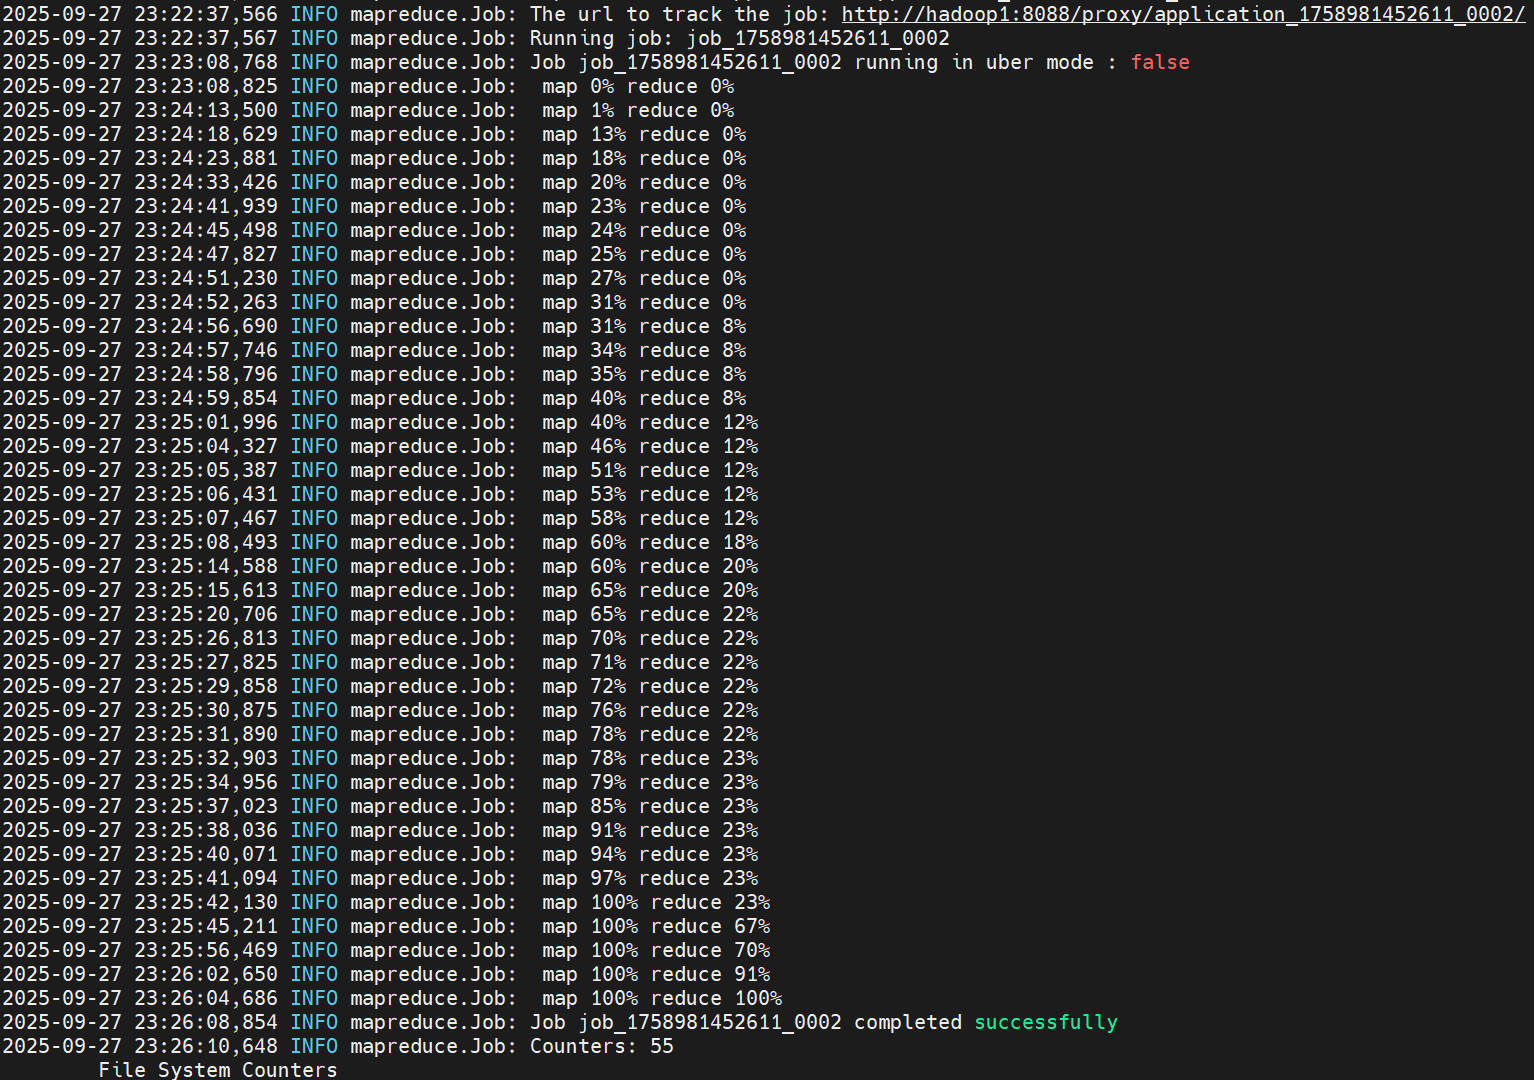
\includegraphics[width=0.9\linewidth]{figures/success.jpg}
  \caption{运行进度显示}
  \label{fig:mapreduce_result}
\end{figure}
可以看到,MapReduce作业已经成功完成,所有的map任务和reduce任务均已成功执行。

\subsection{结果验证}

\begin{lstlisting}[style=shell]
  hbase shell
  create 'InvertedIndexTable', 'fileInfo'
  list
\end{lstlisting}

\begin{figure}[H]
  \centering
  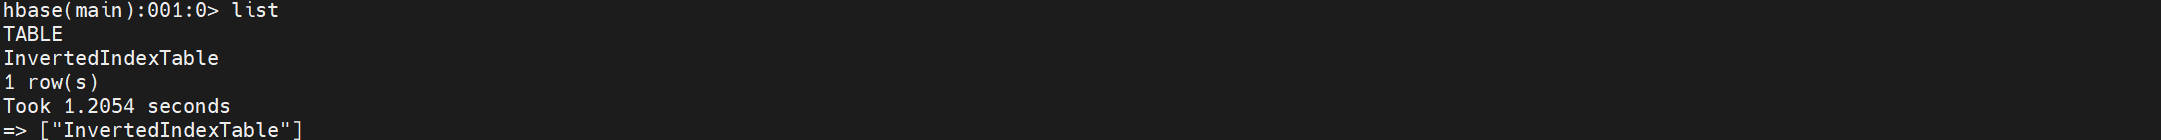
\includegraphics[width=0.9\linewidth]{figures/hbase_list.jpg}
  \caption{HBase Shell中list命令查询表结果}
  \label{fig:hbase_scan}
\end{figure}

可以看到,表InvertedIndexTable已经成功创建。

\lstinline[style=shell]|scan 'InvertedIndexTable', {STARTROW => 'good', LIMIT => 10}|
\begin{figure}[H]
  \centering
  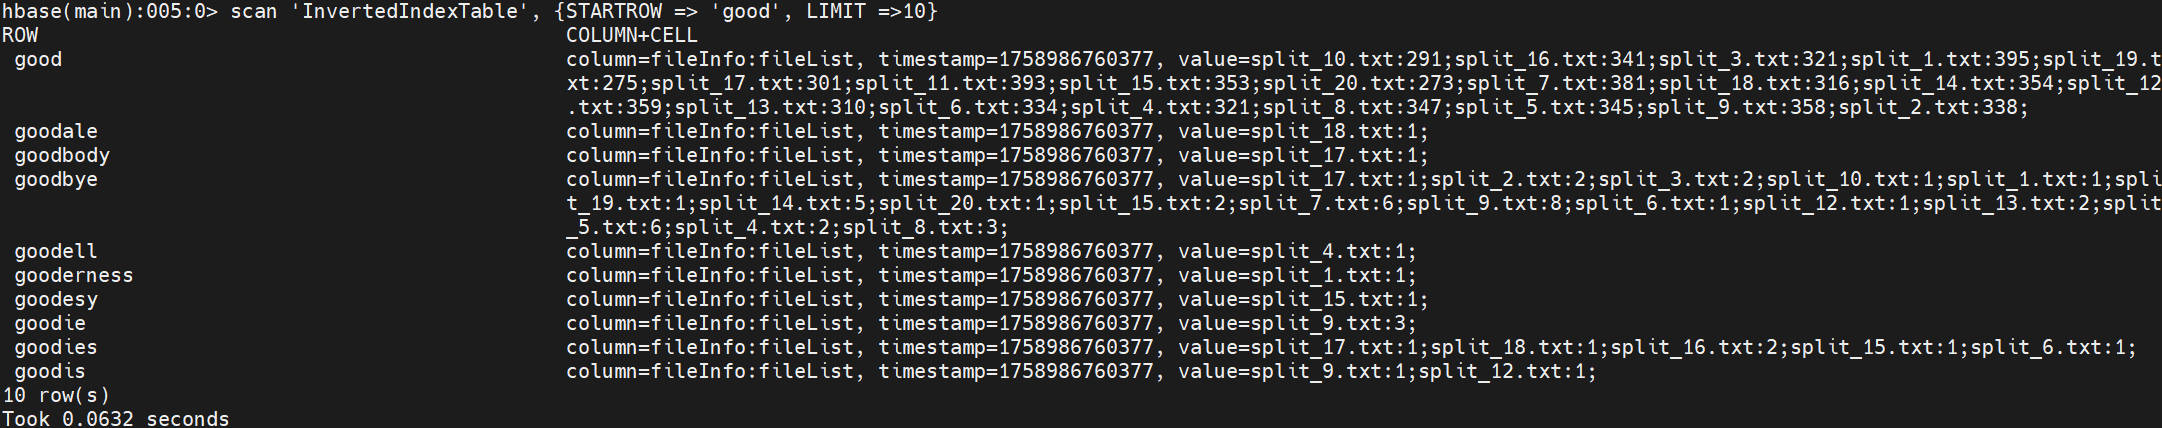
\includegraphics[width=0.9\linewidth]{figures/hbase_scan.jpg}
  \caption{HBase Shell中scan命令查询以'good'开头的单词结果}
  \label{fig:hbase_scan}
\end{figure}
可以看到,以单词'good'开头的单词及其所在的文件编号已经成功存入HBase表中。

\begin{lstlisting}[style=shell]
  get 'InvertedIndexTable', 'hello'
  get 'InvertedIndexTable', 'world'
\end{lstlisting}
\begin{figure}[H]
  \centering
  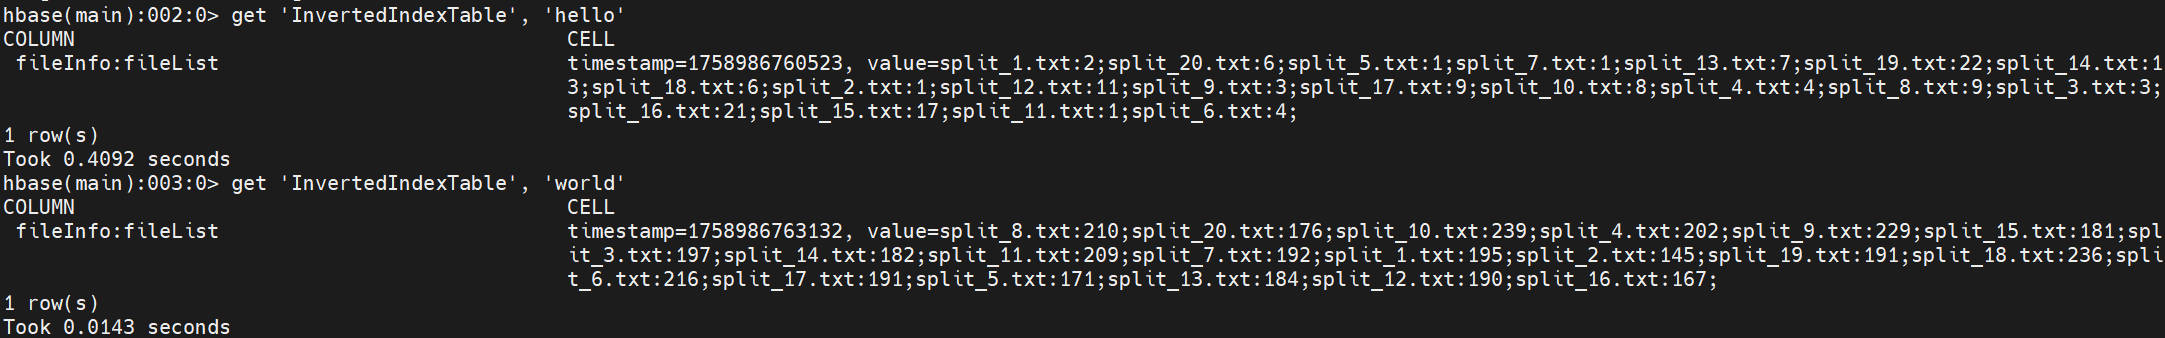
\includegraphics[width=0.9\linewidth]{figures/hbase_get.jpg}
  \caption{HBase Shell中get命令查询结果}
  \label{fig:hbase_get}
\end{figure}
可以看到,单词'hello'和单词'world'均成功存入HBase表中,并且其所在的文件编号也正确无误。

\subsection{性能分析}
本次实现在伪分布式和完全分布式两种模式下均进行了测试。我们搭建的伪分布式环境为一台机器完成所有任务,而完全分布式环境共有三台机器,一台机器作为namenode,另外两台机器作为datanode。

该mapreduce任务分别在两种环境下运行,记录任务的执行时间。伪分布式模式下,任务执行时间为143min,而在完全分布式模式下,任务执行时间只需54min。

在小数据集下,伪分布式模式与完全分布式模式的差异并不明显,但随着数据量的增大,完全分布式模式的高效率,高性能优势将会愈发明显,从而体现出分布式计算的强大能力。

由此看出,分布式计算能够有效提升大数据处理的效率,充分发挥多节点协同工作的优势。

\section{遇到的问题及解决方案}

在运行mapruduce作业时,reduce 任务因执行超时,被应用程序管理器终止,进而导致任务失败。

\lstinline[style=shell]{AttemptID:attempt_1758803251058_0001_r_000000_1 task timeout set: 600s, taskTimedOut: true; task stuck timeout set: 600s, taskStuck: false}

查看日志发现暂停来自主机层面的资源瓶颈。磁盘分区使用率达到了 89 \% ,导致系统写入临时文件失败、应用程序因缺乏磁盘空间无法正常运行。

\begin{figure}[H]
  \centering
  
\includegraphics[width=0.8\linewidth]{figures/disk_usage.jpg}
  \caption{磁盘使用率过高}
\end{figure}

查阅资料后,发现主节点任务多,可以通过增大硬盘容量来解决该问题。
命令行操作如下:

\begin{lstlisting}[style=shell]
sudo fdisk -l # 查看当前磁盘分区
sudo fdisk /dev/sdb # 选择需要扩展的磁盘
partprobe /dev/sda # 让内核重新读取分区表
pvcreate /dev/sda3 # 创建物理卷
vgextend centos /dev/sda3 # 扩展卷组
lvextend /dev/centos/root /dev/sda3 # 扩展逻辑卷
resize2fs /dev/centos/root # 扩展文件系统
df -h # 查看扩展结果
\end{lstlisting}

最后得到:
\lstinline[style=shell]{/dev/mapper/centos-root   31G   15G   17G   46% }
可见磁盘扩展成功,问题得到解决。


\section{总结与心得}
\subsection{实验总结}

本次实验是一次较为完整的大数据系统开发实践,从分布式环境搭建到应用程序实现再到结果验证,涵盖了大数据处理的主要环节。通过这次实验,我们不仅验证了 Hadoop 生态系统的可行性和强大功能,还进一步加深了对分布式计算与存储模式的理解。

在环境搭建方面,我们首先利用 VMware 平台克隆虚拟机,建立了一个三节点的分布式实验环境。在每个节点上,我们手动配置了静态 IP 地址、主机名和 \texttt{/etc/hosts} 文件映射,并设置 SSH 免密登录,确保节点之间能够顺畅通信。这些操作虽然繁琐,但却让我们对分布式系统的运行依赖有了更加直观的体会:一个小小的配置错误,例如 IP 地址冲突或主机名映射遗漏,都可能导致整个集群无法启动。这一过程强化了我们在工程实践中“细节决定成败”的认识。

在框架部署方面,我们成功安装并配置了 Hadoop、ZooKeeper 和 HBase。通过修改 \texttt{core-site.xml}、\texttt{hdfs-site.xml}、\texttt{yarn-site.xml} 等核心配置文件,我们明确了 HDFS 的存储目录、副本数量以及 YARN 的资源调度参数。随后配置的 ZooKeeper 集群为分布式协调提供了可靠支撑,而 HBase 的安装与配置使得我们能够基于 HDFS 存储实现高效的 NoSQL 查询。经过一系列调试与测试,最终集群能够稳定运行,并支持大数据存储与计算任务。

在应用实现方面,我们基于 MapReduce 编程模型完成了倒排索引的构建。通过对原始数据集进行分片处理,使任务能够被合理地分配到不同节点执行。在 Mapper 阶段,我们完成了文本分词与键值对的生成;在 Reducer 阶段,则对分词结果进行聚合统计,并最终写入 HBase 数据库中。实验过程中,我们通过 HDFS Web UI、YARN 任务管理界面以及 HBase Shell 进行了结果验证,确认了倒排索引的正确性与完整性。

在实验结果分析中,我们还对比了伪分布式与完全分布式环境下任务执行时间的差异。结果表明,随着节点数量的增加,MapReduce 任务的执行效率显著提升,充分体现了分布式架构在可扩展性与性能提升方面的优势。这一结果不仅符合我们对分布式系统的理论认知,也进一步证明了 Hadoop 生态在大规模数据处理中具有重要应用价值。

总的来说,本次实验实现了从系统搭建到应用开发的全流程验证,最终顺利完成了倒排索引的构建任务。更为重要的是,实验让我们真正理解了大数据系统各个组件之间的协作关系,以及分布式计算环境下进行应用开发的挑战与价值,为后续进一步研究与实践打下了坚实基础。


\subsection{心得体会}

通过本次实践,我们在分布式计算的理解、系统调试的能力以及团队协作的意识上都有了明显的提升。整个实验的过程不仅仅是简单地完成一系列任务,更是一种综合能力的训练。

在技术层面上,我们对分布式计算原理的理解得到了加深。实验中小组成员亲身经历了从单机环境到多节点集群的转变,体会到 MapReduce 编程模型“分而治之”的思想。Mapper 负责对大规模数据进行分割处理,Reducer 负责结果的聚合与统计,这种任务拆解方式显著提升了计算效率。通过运行实际任务,我们感受到分布式系统的核心价值:并行性、扩展性与容错性。在真实环境下,即使某个节点出现问题,集群依旧能够通过副本机制保证数据的可靠性,这使我们对分布式系统的健壮性有了更深刻的体会。

在工程实践层面上,实验让我们认识到系统配置和调试的重要性。起初我们遇到过多种问题,例如节点间 SSH 无法免密登录、ZooKeeper 配置不一致导致服务无法启动、HBase 无法正常连接 HDFS 等。这些问题迫使我们仔细检查每一个配置文件,并通过日志分析、逐步排错的方式找到并解决问题。这一过程虽然耗时,但极大提升了我们独立解决复杂问题的能力,也让我们学会了如何在工程实践中保持耐心与细心。

在团队协作层面上,本次实验同样带来了深刻的收获。由于实验涉及的环节较多,从虚拟机环境的搭建、集群的配置,到 MapReduce 程序的实现与调试,每个阶段都需要小组成员之间的紧密配合。我们通过合理分工、及时沟通与相互检查,保证了实验能够顺利推进。这让我们意识到,分布式系统的学习与开发不仅仅是技术问题,更是协作与组织问题。良好的沟通与分工机制,往往能在关键时刻提高效率,避免重复劳动和错误。

综合来看,本次实验不仅帮助我们掌握了 Hadoop、ZooKeeper 和 HBase 的基本使用方法,还加深了对大数据系统整体架构的理解。在未来的学习与科研中,这些宝贵的经验将为我们应对更加复杂的工程实践提供坚实的支持。同时,实验中形成的系统化思维方式和团队合作意识,也将成为我们小组在后续研究和开发工作中的重要财富。


% --- 参考文献 ---
\printbibliography[heading=bibliography,title=参考文献]

\end{document}